As mentioned at the beginning of chapter 4, the analysis is designed for maximum sensitivity to the SUSY simplified model T2tt, T1tttt, T1ttbb, T5tttt and T5ttcc topology resulting in final states with multiple top quarks, hence multiple jets and b-tagged jets, produced in top squark decay, no leptons, and large \MET. The T2tt, T5ttcc and T1tttt final states differ in the number of jets, b-tagged jets and top quarks produced. 

Targeting the above-mentioned final states, the data are initially selected by requiring a minimum number of jets and b-jets (\njets and \nbjets) and large \MET. The search regions are ultimately defined in exclusive bins of \ntops, \nbjets, \HT, \MET and \MTTwo, where \ntops is the number of reconstructed top quarks. SM backgrounds arise from processes such as \ttbar, Z+jets, W/top+jets and QCD multijets with smaller contributions from rare processes.

The data selection process starts with the triggers and follows with a baseline selection and the definition of the search bins. The top quark reconstruction and identification procedure (top tagging) is described in this section, as well as the MC samples that model signal and backgrounds.

\subsection{Trigger}
\label{sec:trig}

The trigger is the first filter applied to the data. We choose \MET based triggers in this analysis instead of the HT based triggers used for the analysis of the 2015 data because of HT bit trigger issues in the 2016 run H data, where Run H corresponds to a data-taking period between September 16 2016 and October 28 2016 consisting of 92.5 fb$^{-1}$ of data. 

The trigger sets are used in this analysis are: a general trigger, described below, used for the search regions and for the estimation of the QCD multijet background and a single-muon trigger for the $Z$+jets background evaluation. We measure the search trigger efficiencies with different orthogonal triggers to check differences in the turn-on behavior. The corresponding efficiencies are applied to correct the simulations used in the analysis.

Six search triggers are used to collect events for this analysis. They are seeded by \MET in the Level-1 trigger. 
\begin{itemize}
\item \texttt{ HLT\_PFMET100\_PFMHT100\_IDTight\_v*}
\item \texttt{ HLT\_PFMET110\_PFMHT110\_IDTight\_v*}
\item \texttt{ HLT\_PFMET120\_PFMHT120\_IDTight\_v*}
\item \texttt{ HLT\_PFMETNoMu100\_PFMHTNoMu100\_IDTight\_v*} 
\item \texttt{ HLT\_PFMETNoMu110\_PFMHTNoMu110\_IDTight\_v* }
\item \texttt{ HLT\_PFMETNoMu120\_PFMHTNoMu120\_IDTight\_v*}
\end{itemize}

The probability for these triggers to accept events (trigger efficiency) is measured in a sample of events collected by the single-electron trigger
\begin{itemize}
  \item \texttt{HLT\_Ele27\_WPTight\_v*},
\end{itemize}
which has been commonly used within CMS for the \MET trigger efficiency measurement. Events from the single electron dataset are also required to have at least one offline reconstructed electron with $p_{T}>$ 30 GeV. These selection criteria ensure that the single electron trigger is efficient. 

To measure the search trigger efficiency, additional requirements to mimic the baseline selection, defined in Sec.~\ref{sec:baselineselection}, are imposed.
\begin{itemize}
  \item Satisfy all filters
  \item Veto reconstructed muon
  \item $\njets\geq4$
  \item \nbjets $\ge$ 1
  \item \HT $\ge$ 300 GeV
  \item $\Delta\phi(\MET, j_{1,2,3})>$ 0.5, 0.5, 0.3
\end{itemize}

The efficiency of the search triggers is measured as a function of the offline \MET. Events satisfying the above requirements are defined as the
denominator, while events satisfying these criteria that are also selected by the search triggers are defined as the numerator. It has been found that the \MET trigger efficiency has a non-trivial dependency on the offline $\HT$. The search trigger efficiencies are measured in the low $\HT$ (300 $< \HT <$ 1000) and high
$\HT$ ($\HT >$ 1000) region, as shown in Fig.~\ref{fig:TrigMET}.
\begin{figure}[tbp]
 \begin{center}
   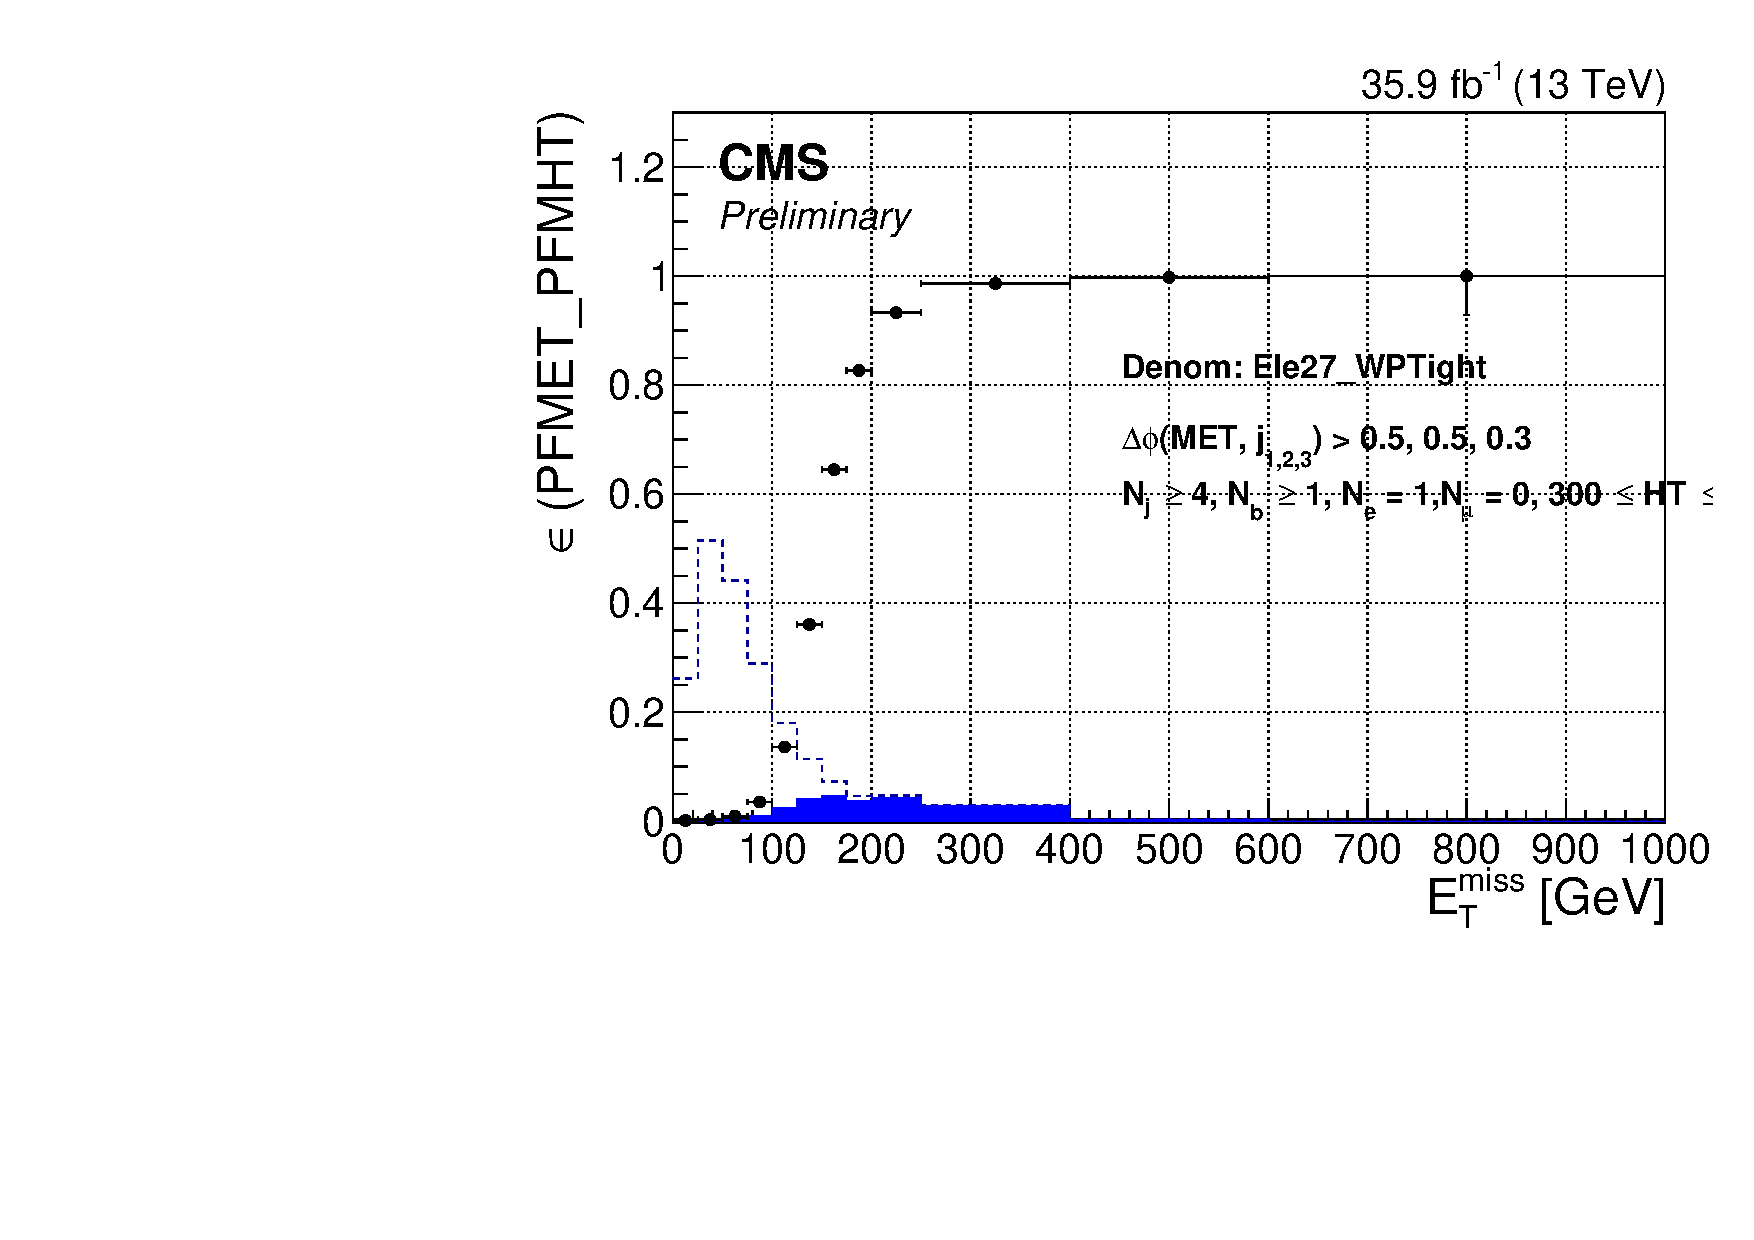
\includegraphics[width=0.49\linewidth]{sections/mc4/EvtSelSBOpt/figures/TrigEle_Stop_TrigMET_HTLess1000_9.pdf}
   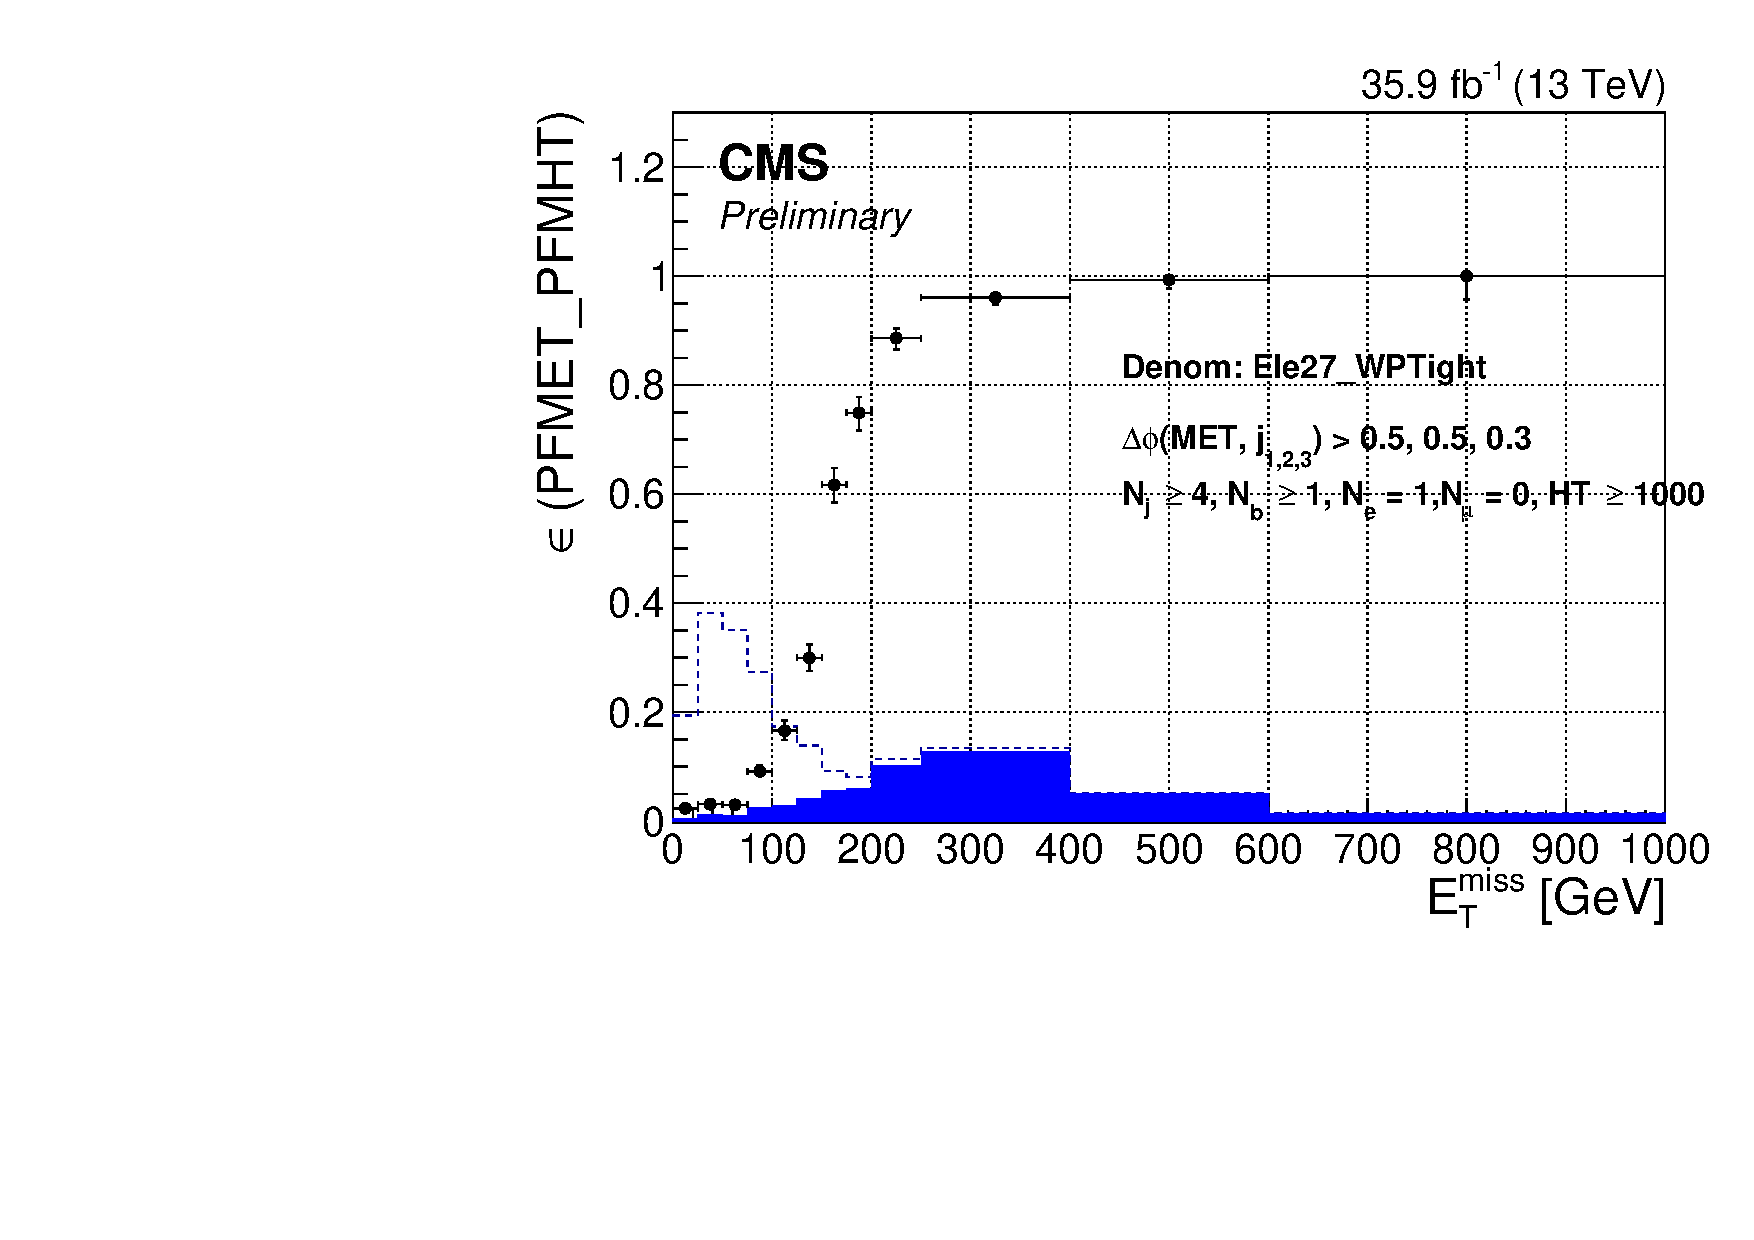
\includegraphics[width=0.49\linewidth]{sections/mc4/EvtSelSBOpt/figures/TrigEle_Stop_TrigMET_HTMore1000_9.pdf}
   \caption{ The trigger efficiency, denote by the black point, as a function
   of the offline \MET for (left) 300 $< \HT <$ 1000 and (right) $\HT >$ 1000.
   The error bar indicates the statistical uncertainty of the trigger
   efficiency. The dash blue line represents the denominator passing the
   selection, while the solid blue histogram represents the numerator where
   the denominator events also trigger the search triggers. }
   \label{fig:TrigMET}
 \end{center}
\end{figure}

Besides measuring the \MET trigger efficiency from the single electron dataset, the trigger efficiency can be measured from a single muon and HTMHT dataset. To account for possible bias from different measurements, we take the measurement from the single-electron dataset as the nominal one, and the variation from the measurements from single-muon and HTMHT dataset as the systematic uncertainty in the trigger efficiency, as shown Fig~\ref{fig:TrigMETSys}. For \MET above 250 GeV, we observe similar \MET trigger efficiencies, with a systematic uncertainty less than 1\%.

For the \MET trigger efficiency measured from the single-muon dataset, events are collected with the single-muon trigger
\begin{itemize}
  \item \texttt{HLT\_Mu50\_v*},
\end{itemize}
with the following offline requirements:
\begin{itemize}
  \item Satisfy all filters
	\item Leading reconstructed muon has $p_{T}>$ 50 GeV
  \item Veto reconstructed electron
  \item $\njets\geq4$
  \item \nbjets $\ge$ 1
  \item \HT $\ge$ 300 GeV
  \item $\Delta\phi(\MET, j_{1,2,3})>$ 0.5, 0.5, 0.3
\end{itemize}
For the \MET trigger efficiency measured from the HTMHT dataset, events are collected by the HT triggers: 
\begin{itemize}
  \item \texttt{HLT\_PFHT200\_v*},
  \item \texttt{HLT\_PFHT250\_v*},
  \item \texttt{HLT\_PFHT300\_v*},
  \item \texttt{HLT\_PFHT350\_v*},
  \item \texttt{HLT\_PFHT400\_v*},
  \item \texttt{HLT\_PFHT475\_v*},
  \item \texttt{HLT\_PFHT600\_v*},
  \item \texttt{HLT\_PFHT800\_v*},
  \item \texttt{HLT\_PFHT900\_v*},
  \item \texttt{HLT\_CaloJet500\_NoJetID\_v*},
\end{itemize} 
in which \texttt{HLT\_CaloJet500\_NoJetID\_v*} is recommended at Level-1 to recover the inefficiency of the L1\_HTT trigger during period H data taking. Events are required to satisfy the following criteria:
\begin{itemize}
  \item Satisfy all filters
  \item Veto reconstructed electron
  \item Veto reconstructed muon
  \item $\njets\geq4$
  \item \nbjets $\ge$ 1
  \item \HT $\ge$ 300 GeV
  \item $\Delta\phi(\MET, j_{1,2,3})>$ 0.5, 0.5, 0.3
\end{itemize}

\begin{figure}[tbp]
 \begin{center}
   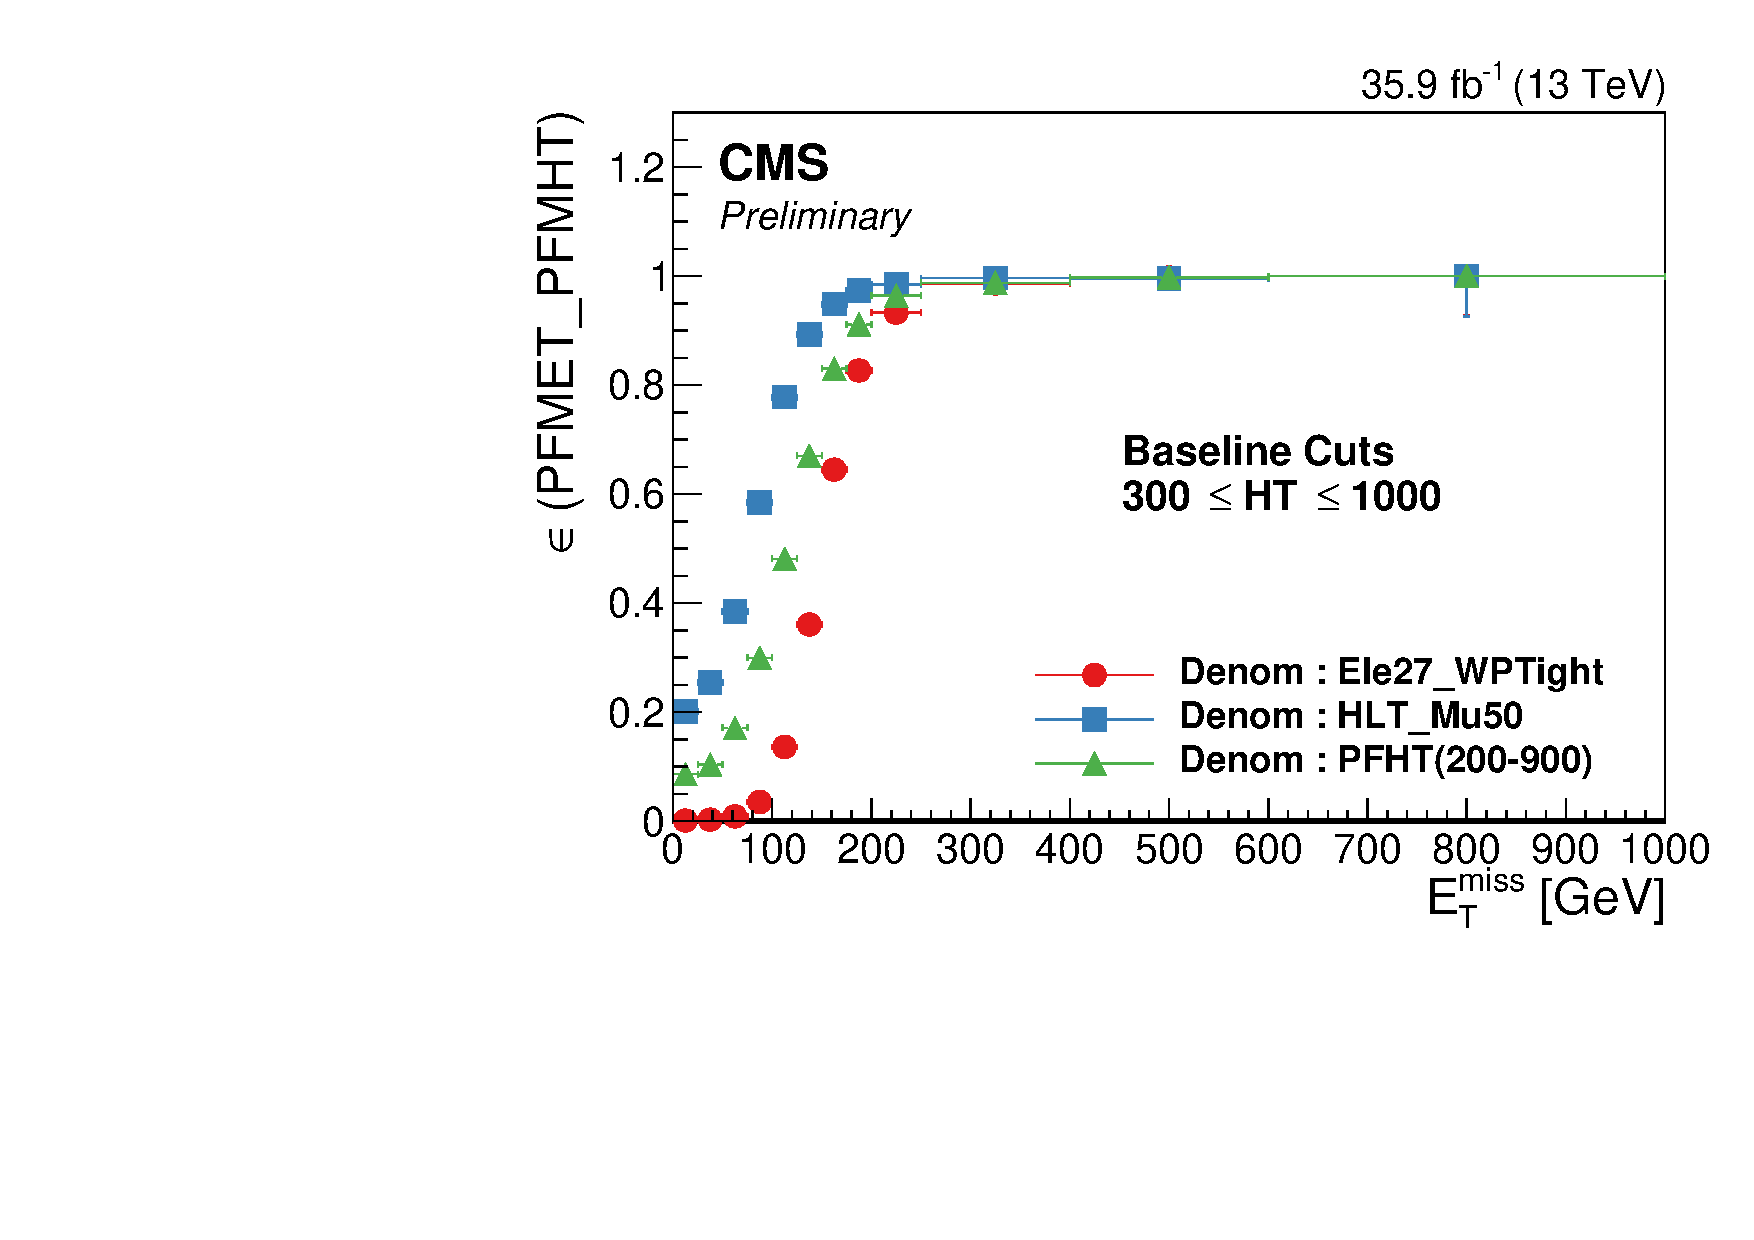
\includegraphics[width=0.49\linewidth]{sections/mc4/EvtSelSBOpt/figures/TrigMET_HTLess1000.pdf}
   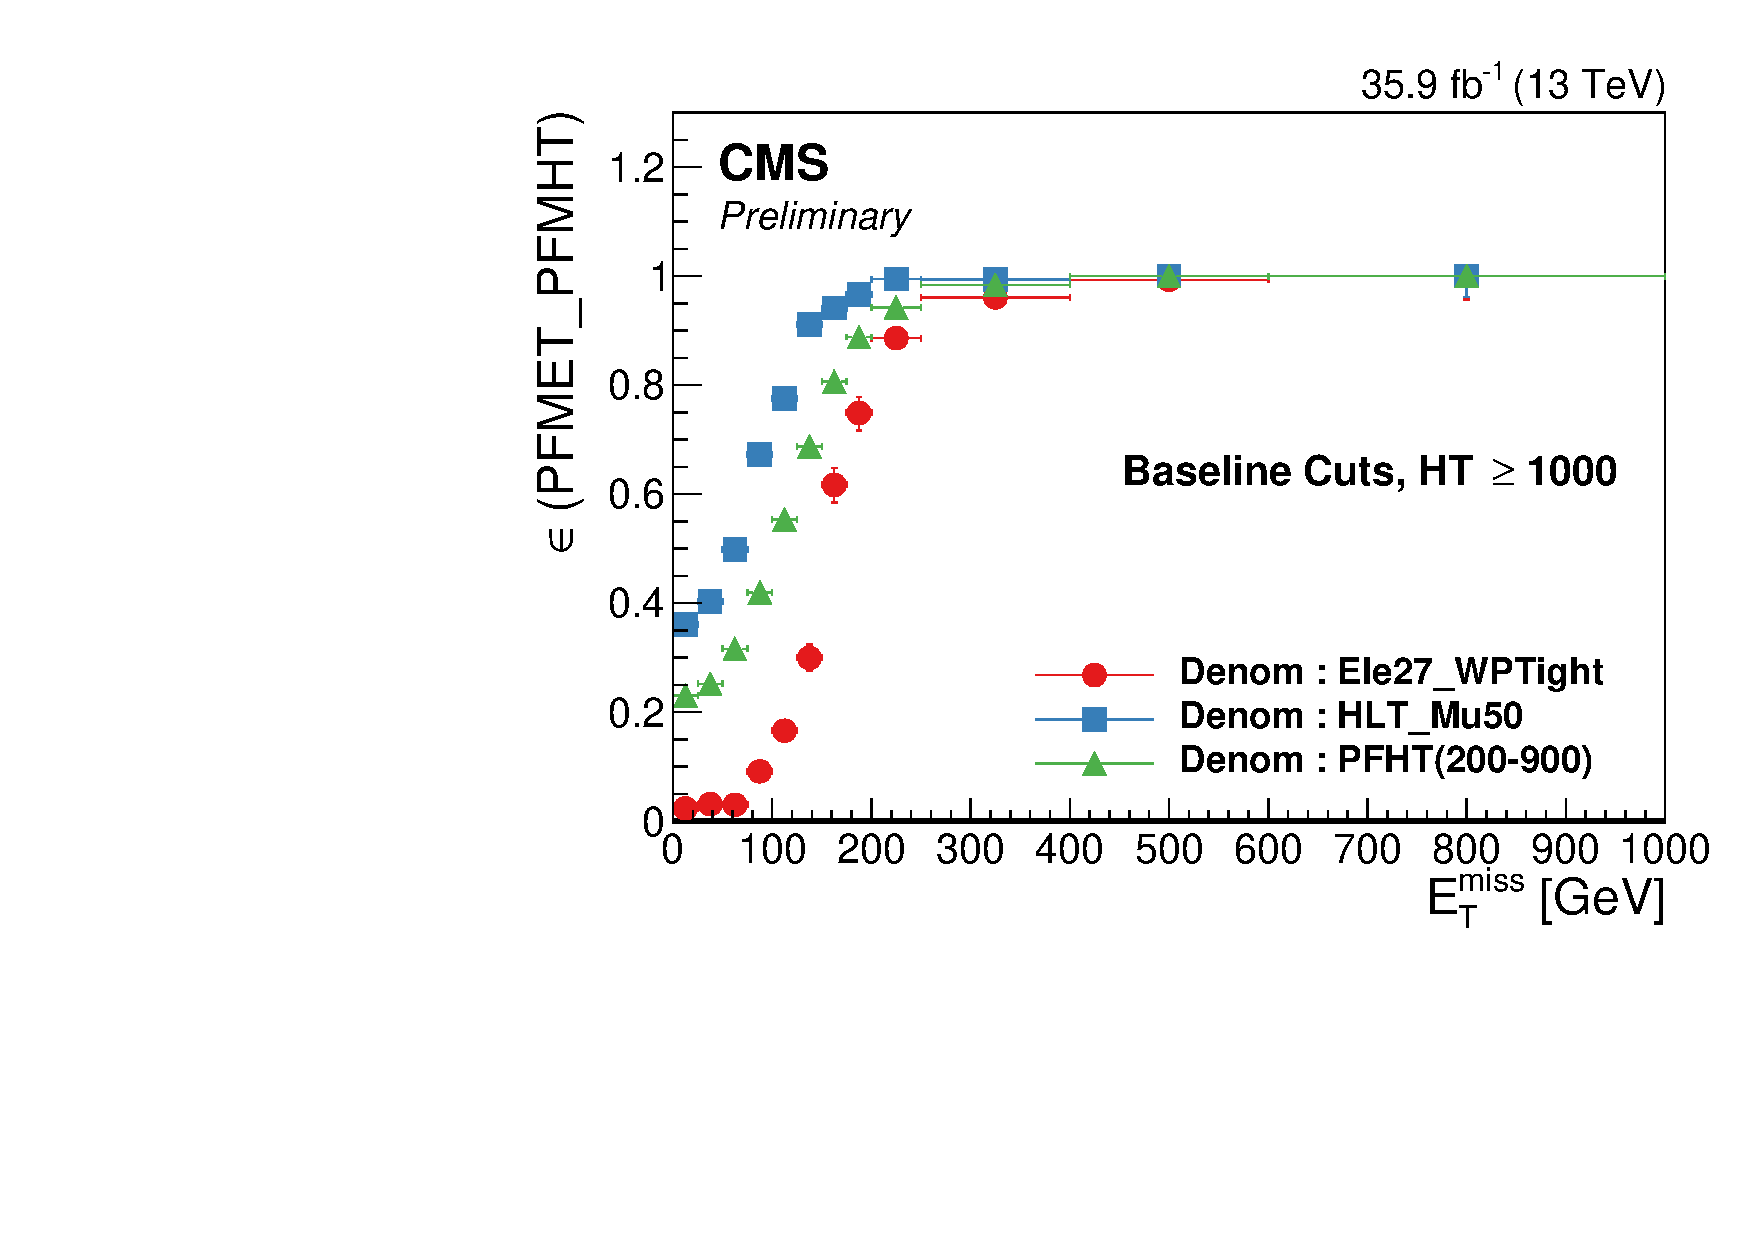
\includegraphics[width=0.49\linewidth]{sections/mc4/EvtSelSBOpt/figures/TrigMET_HTMore1000.pdf}
   \caption{ The trigger efficiency, denote by the black point, as a function
   of the offline \MET for (left) 300 $< \HT <$ 1000 and (right) $\HT >$ 1000.
   The error bar indicates the statistical uncertainty of the trigger
   efficiency. The blue square represents efficiency measured with
   single-muon dataset.  The red point represents efficiency measured
   with single-electron dataset while the green triangle represents
   efficiency measured with HT dataset.}
   \label{fig:TrigMETSys}
 \end{center}
\end{figure}

We also checked the trigger efficiency as a function of number of AK4 jets and $b$-tagged jets, after requiring \MET $>$ 250 GeV, as shown in
Fig~\ref{fig:TrigMETJets}. Similar efficiencies are observed from the different measurements.

\begin{figure}[tbp]
 \begin{center}
   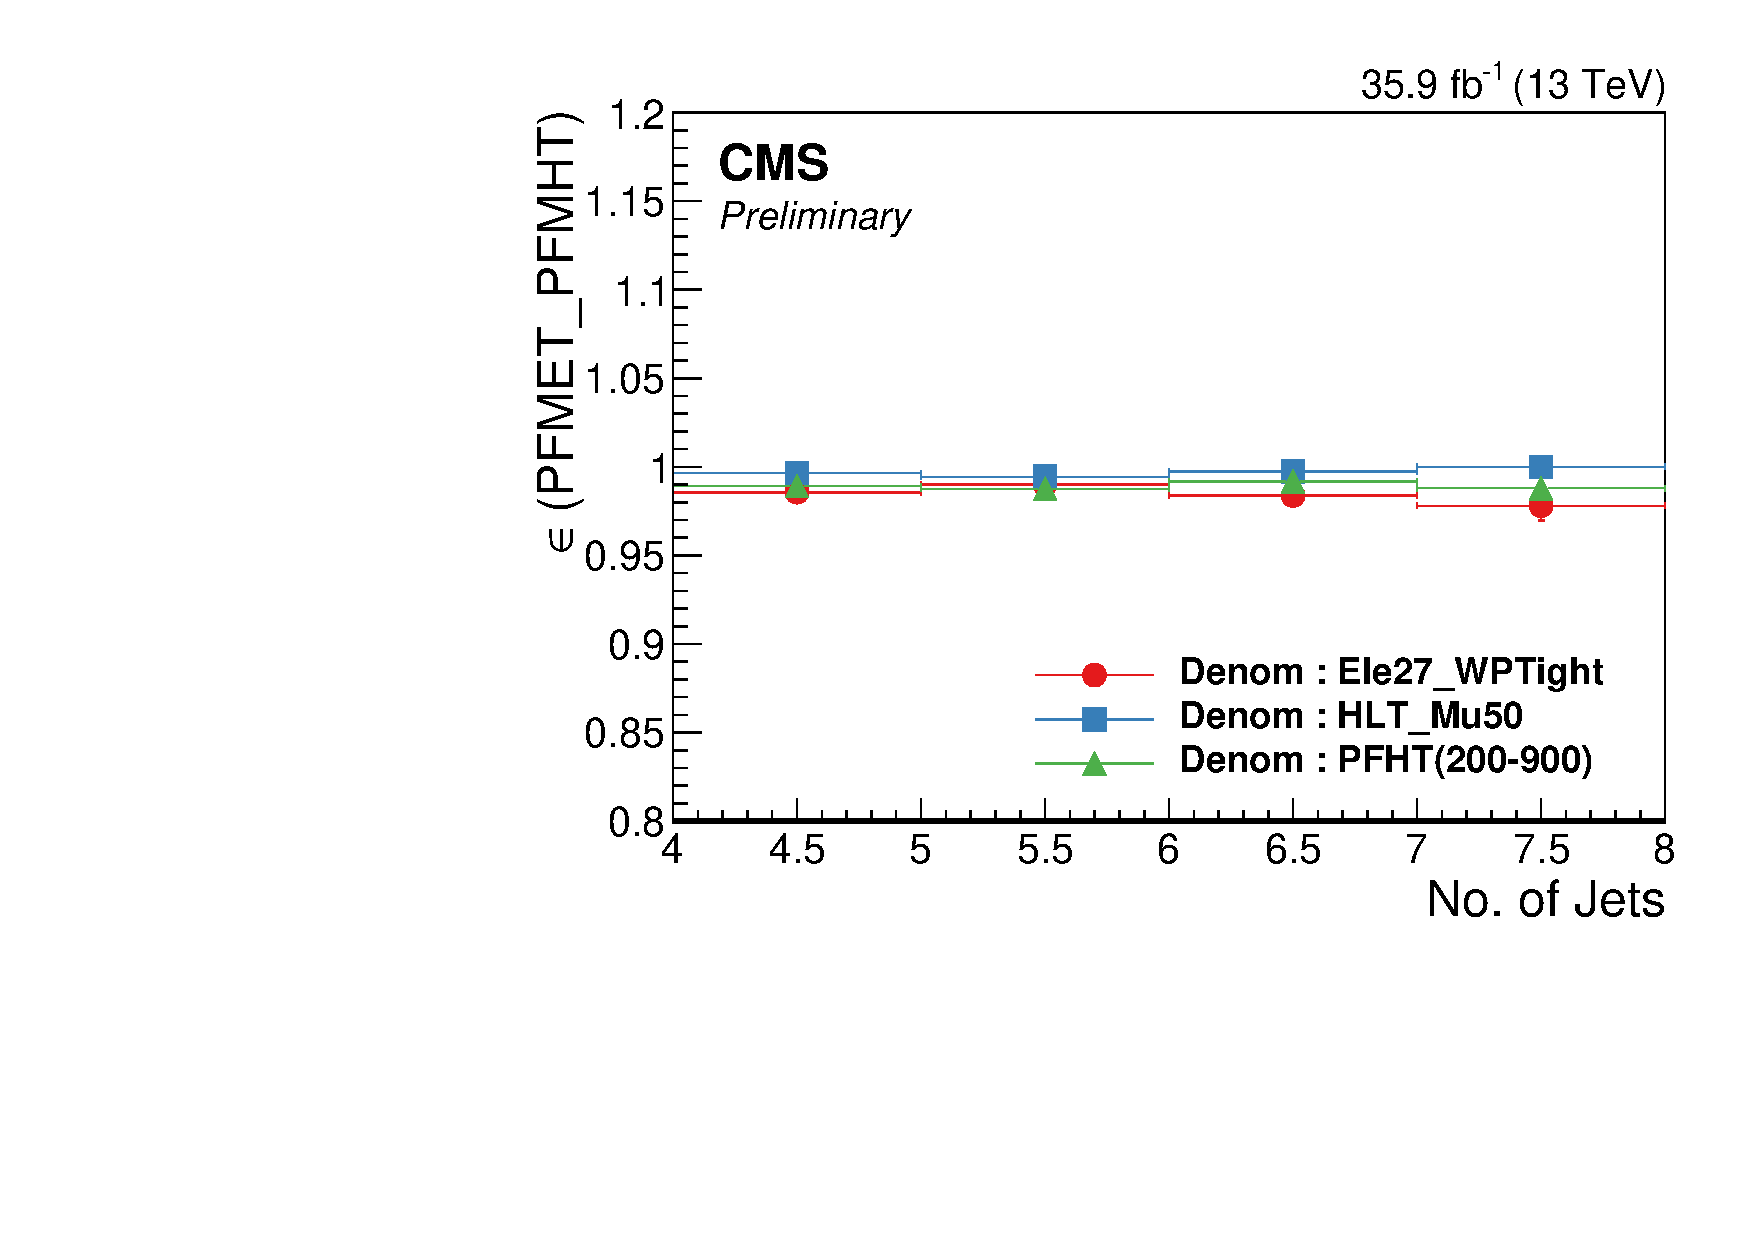
\includegraphics[width=0.49\linewidth]{sections/mc4/EvtSelSBOpt/figures/TrigNJets.pdf}
   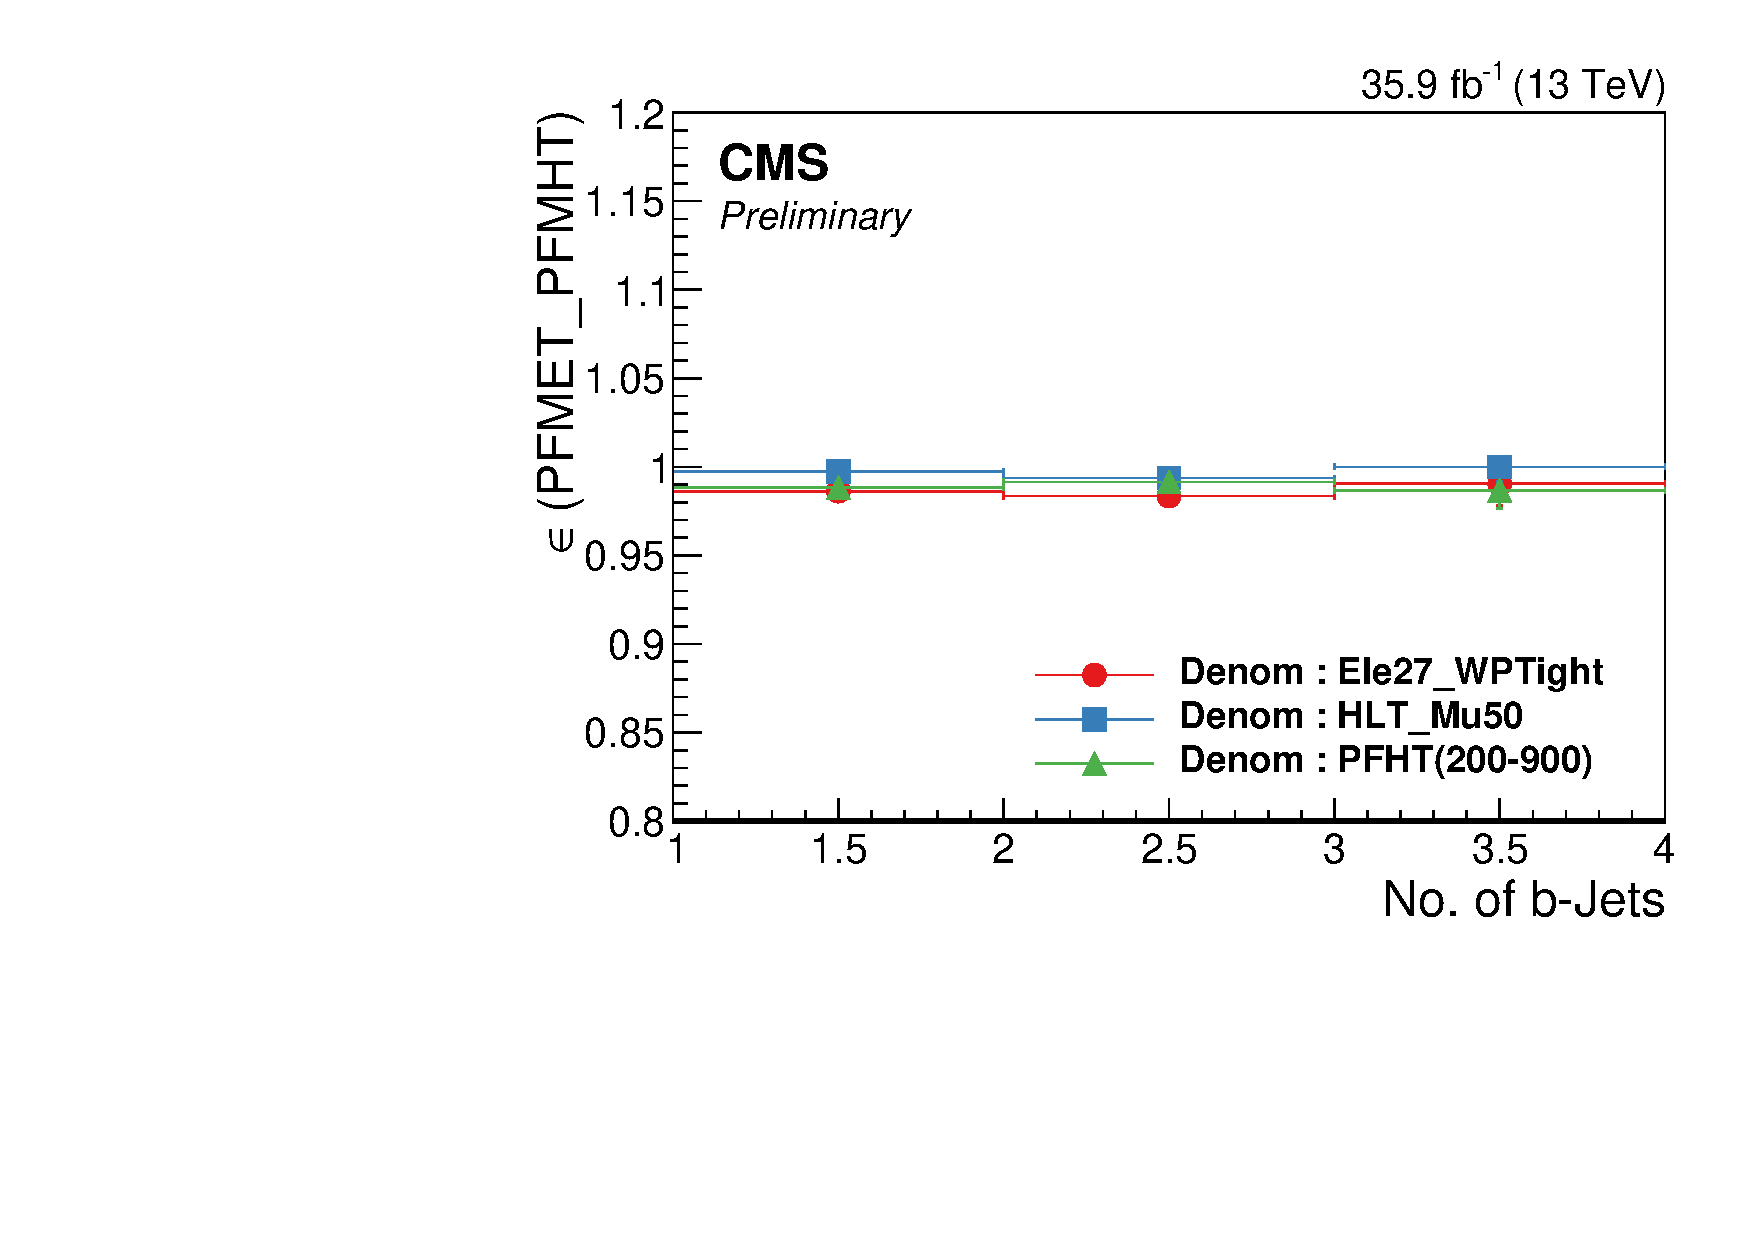
\includegraphics[width=0.49\linewidth]{sections/mc4/EvtSelSBOpt/figures/TrigNBs.pdf}
   \caption{ The trigger efficiency, denote by the black point, as a function
		 of the offline (left) number of jets with $p_{T}>$ 30 GeV and (right) number
		 of $b$-tagged jets with $p_{T}>$ 30GeV. The error bar indicates the
   statistical uncertainty of the trigger efficiency. The blue square
   represents efficiency measured with single-muon dataset.  The red point
   represents efficiency measured with single-electron dataset while the green
   triangle represents efficiency measured with HT dataset.}
   \label{fig:TrigMETJets}
 \end{center}
\end{figure}

The QCD multijet background is estimated using the events triggered by the search triggers, but with offline requirements to select a QCD-enriched region. Since there is usually very little genuine \MET in QCD events, the \MET trigger efficiency in the QCD-enriched region is expected to be different from that of the search region in the low \MET region. A measurement of the trigger efficiency in the QCD-enriched region is performed in the HTMHT dataset to avoid bias. Events are required to satisfy similar criteria as for the search trigger efficiency measurement, except an inverted $\Delta\phi(\MET, j_{1,2,3})$ requirement is imposed:
\begin{itemize}
  \item Satisfy all filters
  \item Veto reconstructed electron
  \item Veto reconstructed muon
  \item $\njets\geq4$
  \item \nbjets $\ge$ 1
  \item \HT $\ge$ 300 GeV
  \item $\Delta\phi(\MET, j_{1,2,3})<$ 0.5, 0.5, 0.3
\end{itemize}
The trigger efficiency is measured as a function of the offline \MET and is shown in Fig~\ref{fig:TrigMETQCD}.
\begin{figure}[tbp]
 \begin{center}
   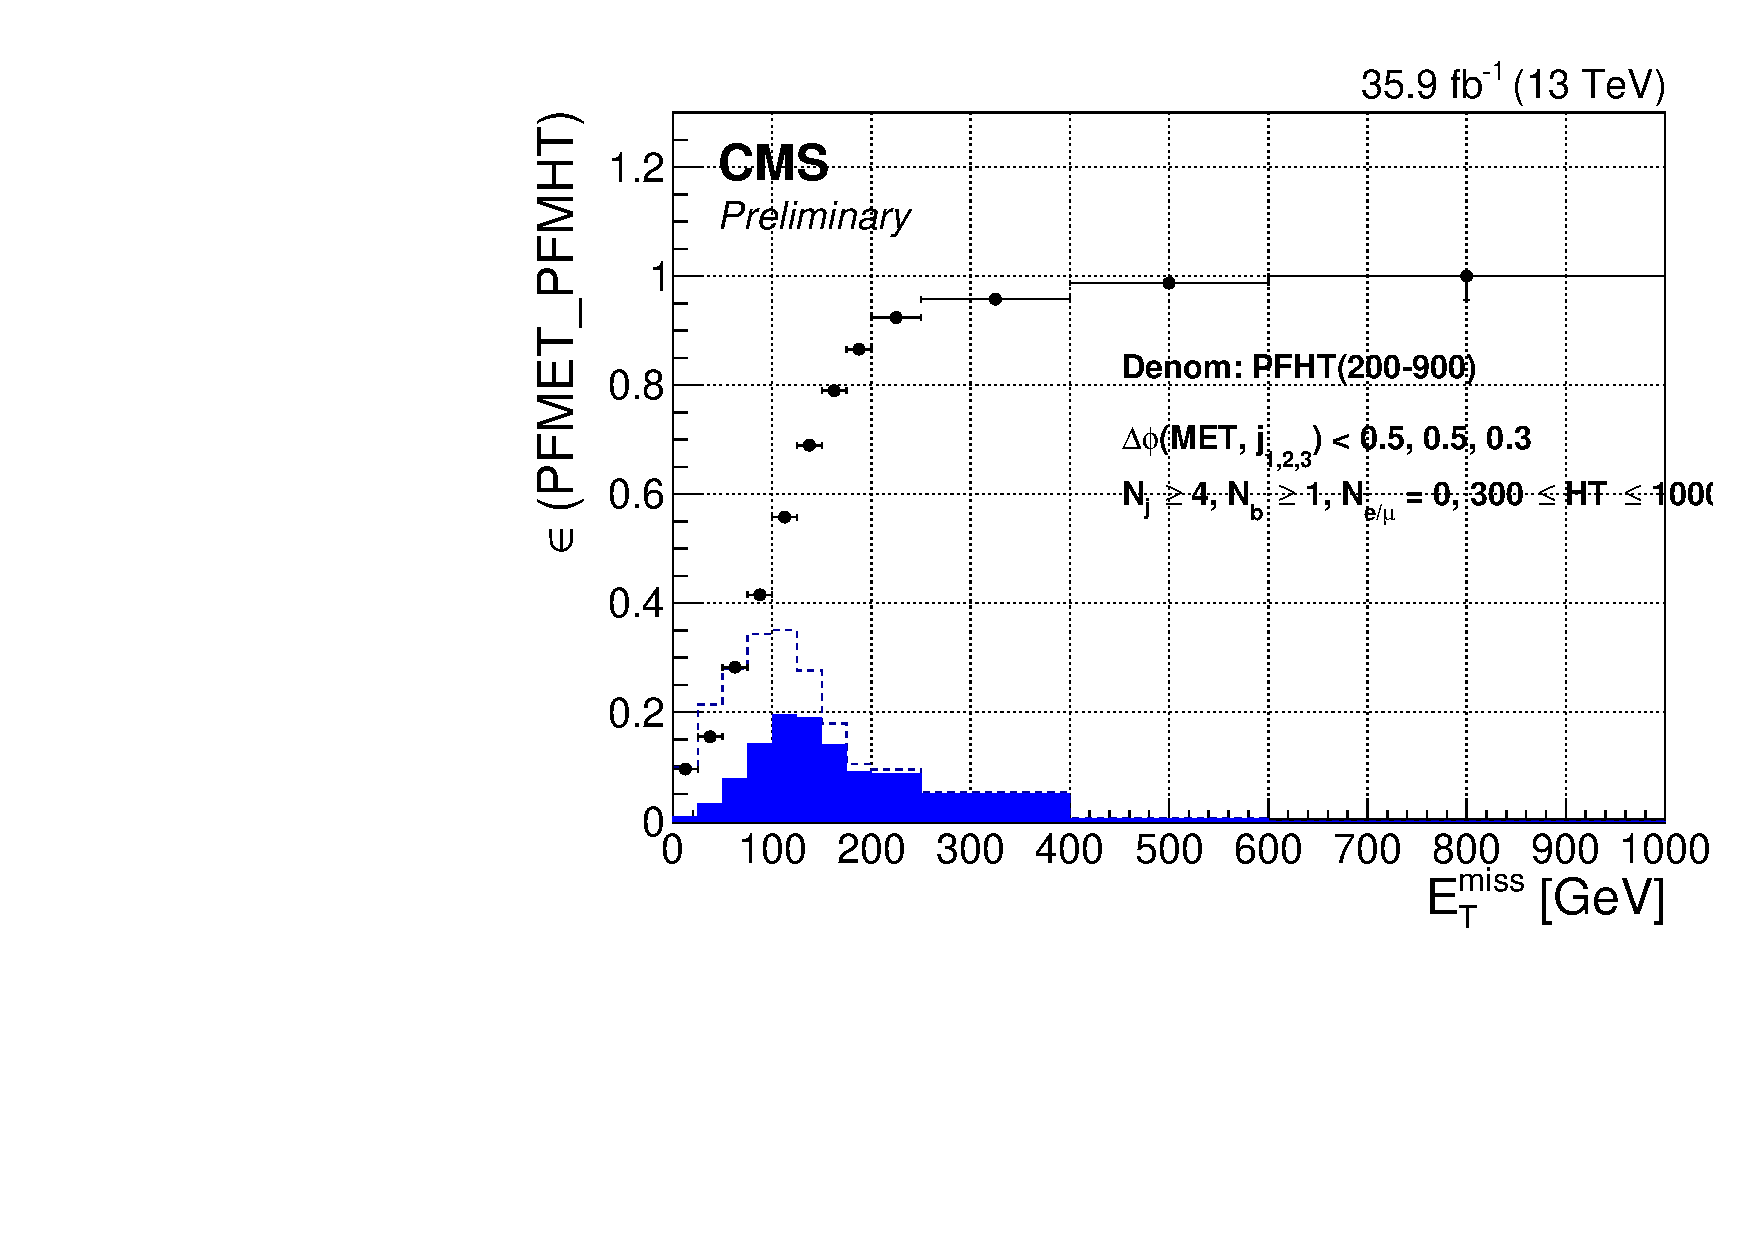
\includegraphics[width=0.49\linewidth]{sections/mc4/EvtSelSBOpt/figures/TrigHT_QCD_TrigMET_HTLess1000_9.pdf}
   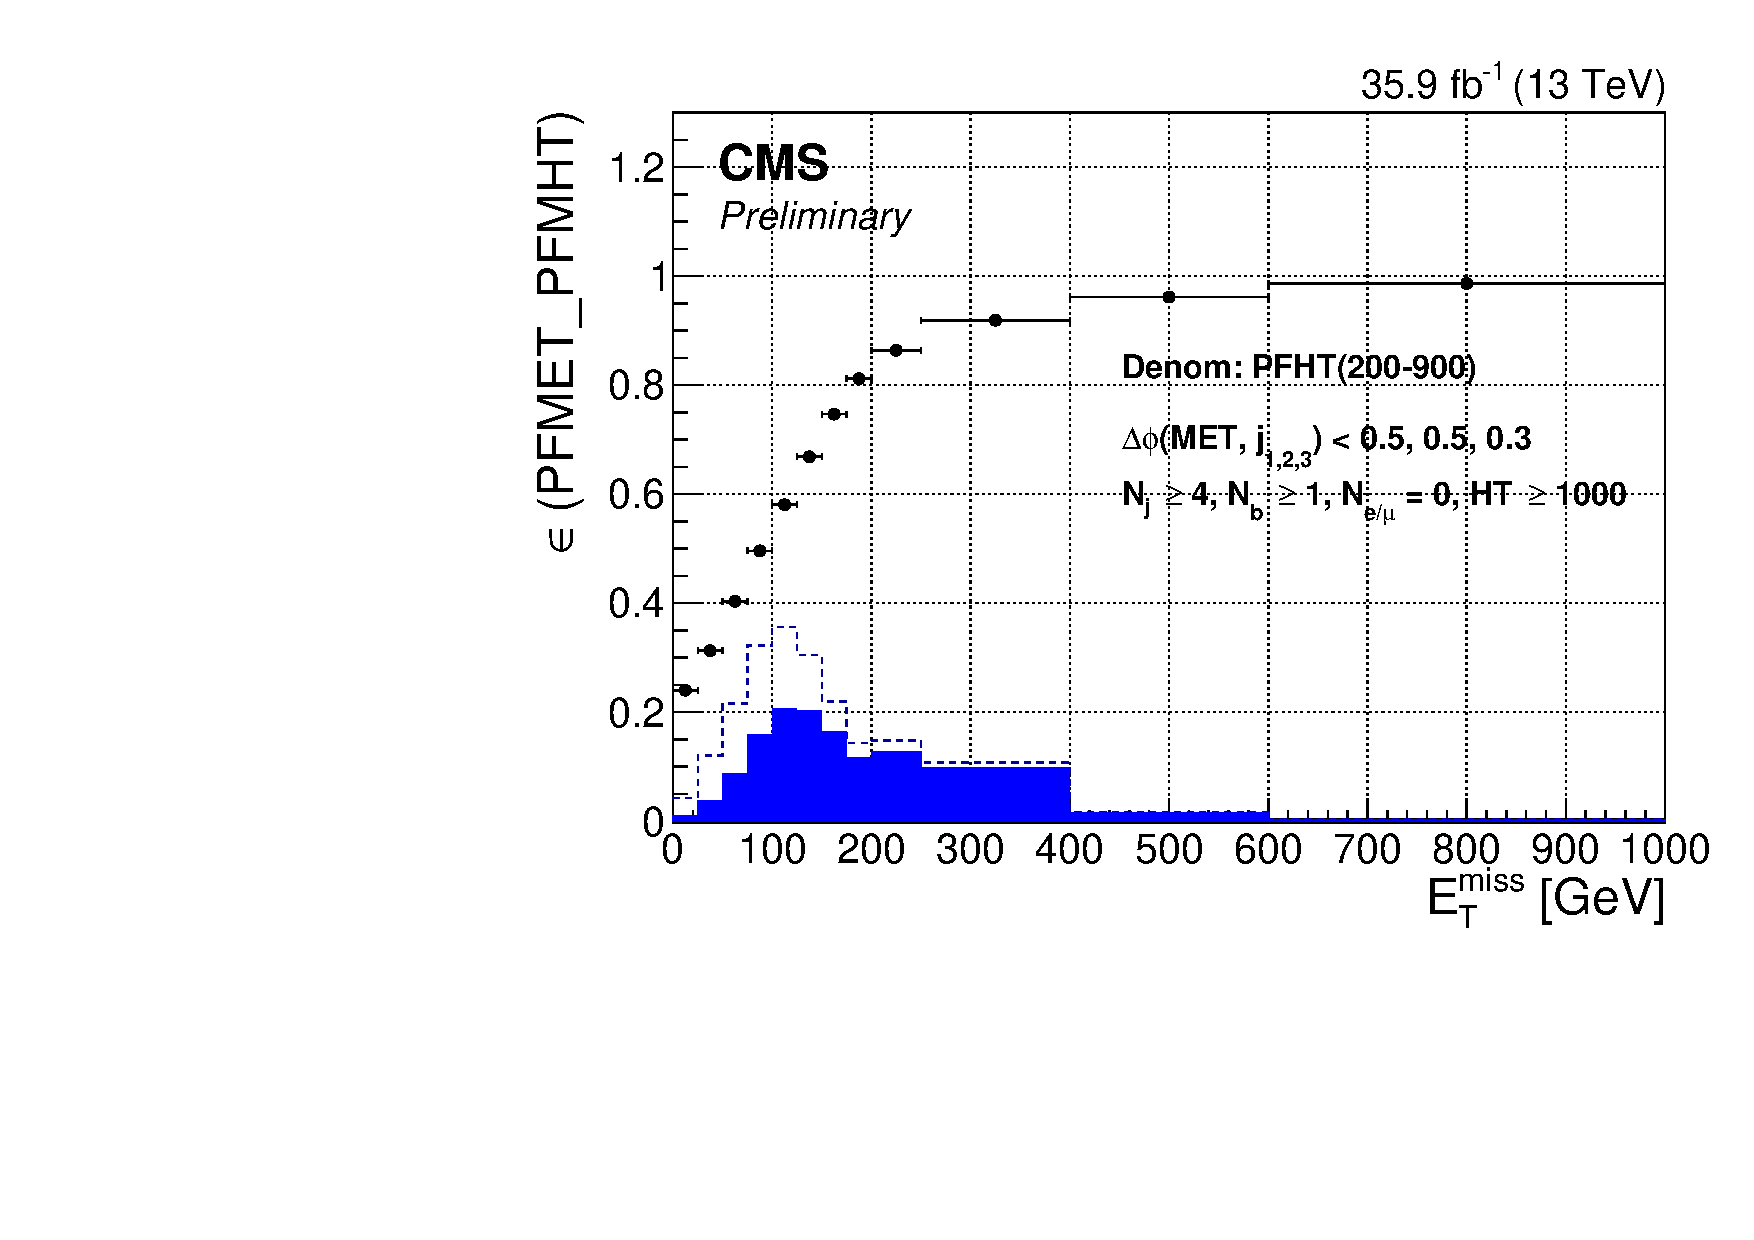
\includegraphics[width=0.49\linewidth]{sections/mc4/EvtSelSBOpt/figures/TrigHT_QCD_TrigMET_HTMore1000_9.pdf}
   \caption{ The trigger efficiency, denote by the black point, as a function
   of the offline \MET for (left) 300 $< \HT <$ 1000 and (right) $\HT >$ 1000.
   The error bar indicates the statistical uncertainty of the trigger
   efficiency. The dash blue line represents the denominator passing the
   selection, while the solid blue histogram represents the numerator where
   the denominator events also trigger the search triggers. }
   \label{fig:TrigMETQCD}
 \end{center}
\end{figure}

Events in the di-muon control sample, which is used for the estimation of the background from events in which a Z boson decays into neutrinos, are collected with the single muon trigger. 
\begin{itemize}
  \item \texttt{HLT\_IsoMu24\_eta2p1\_v*}.
  \item \texttt{HLT\_IsoTKMu24\_eta2p1\_v*}.
  \item \texttt{HLT\_Mu50\_eta2p1\_v*}.
\end{itemize}
The trigger efficiencies are measured in the single-electron sample with the following criteria:
\begin{itemize}
  \item Satisfy all filters
	\item Leading reconstructed electron has $p_{T}>$ 30 GeV
  \item At least one reconstructed muon
  \item $\njets\geq4$
  \item \nbjets $\ge$ 1
  \item \HT $\ge$ 300 GeV
\end{itemize}

The measured single muon trigger efficiency as a function of the reconstructed leading muon $p_{T}$ and $\eta$ is shown in Fig.~\ref{fig:TrigMuon}. The muon trigger efficiency is also measured in the HT and MET dataset as cross checks. We also checked the benefits of adding the double muon triggers: 
\begin{itemize}
  \item \texttt{HLT\_Mu17\_TrkIsoVVL\_Mu8\_TrkIsoVVL\_DZ\_v*}
  \item \texttt{HLT\_Mu17\_TrkIsoVVL\_TkMu8\_TrkIsoVVL\_DZ\_v*}.
\end{itemize}
We do observe a small gain in the muon trigger efficiencies as shown in Fig~\ref{fig:TrigMuon}, but no benefit for the $Z \rightarrow \nu \nu$ background method.

\begin{figure}[tbp]
 \begin{center}
   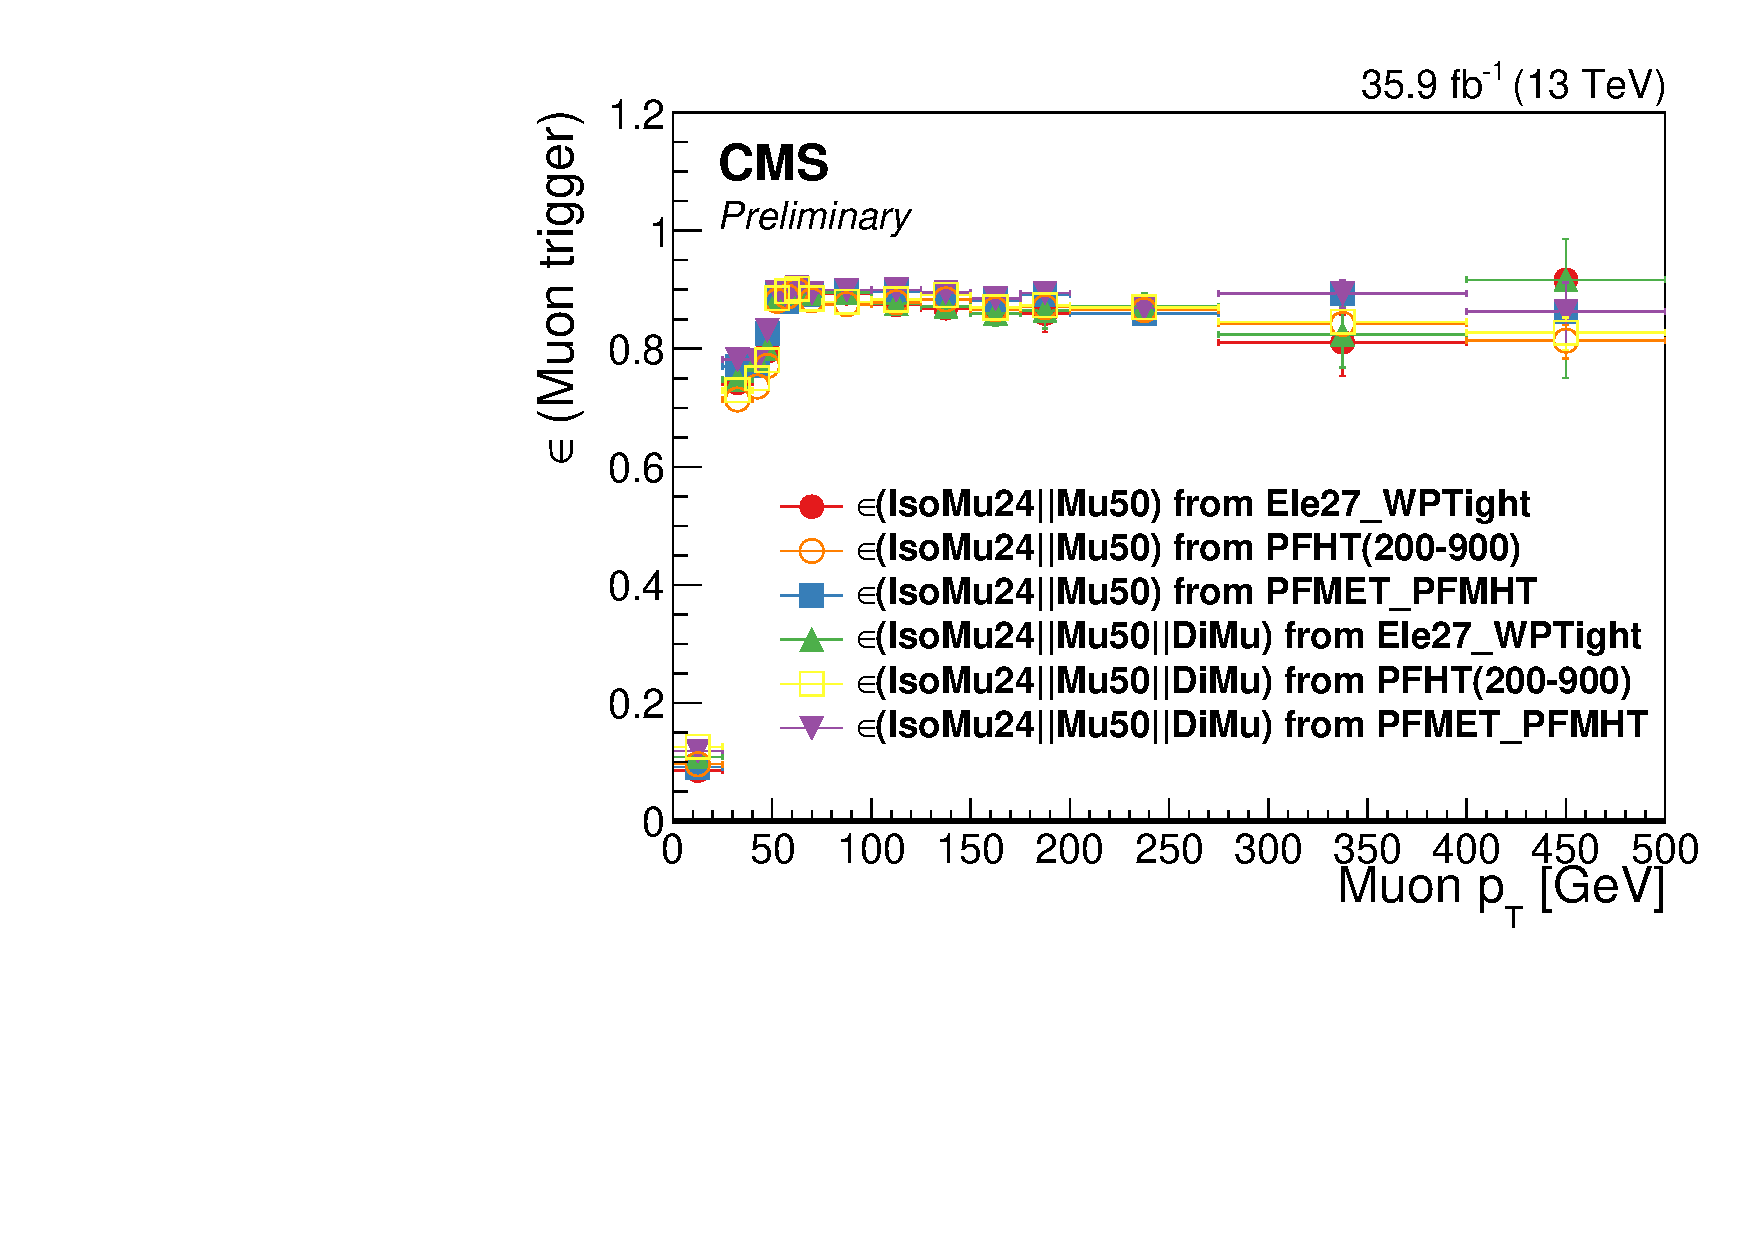
\includegraphics[width=0.49\linewidth]{sections/mc4/EvtSelSBOpt/figures/MuonPT.pdf}
   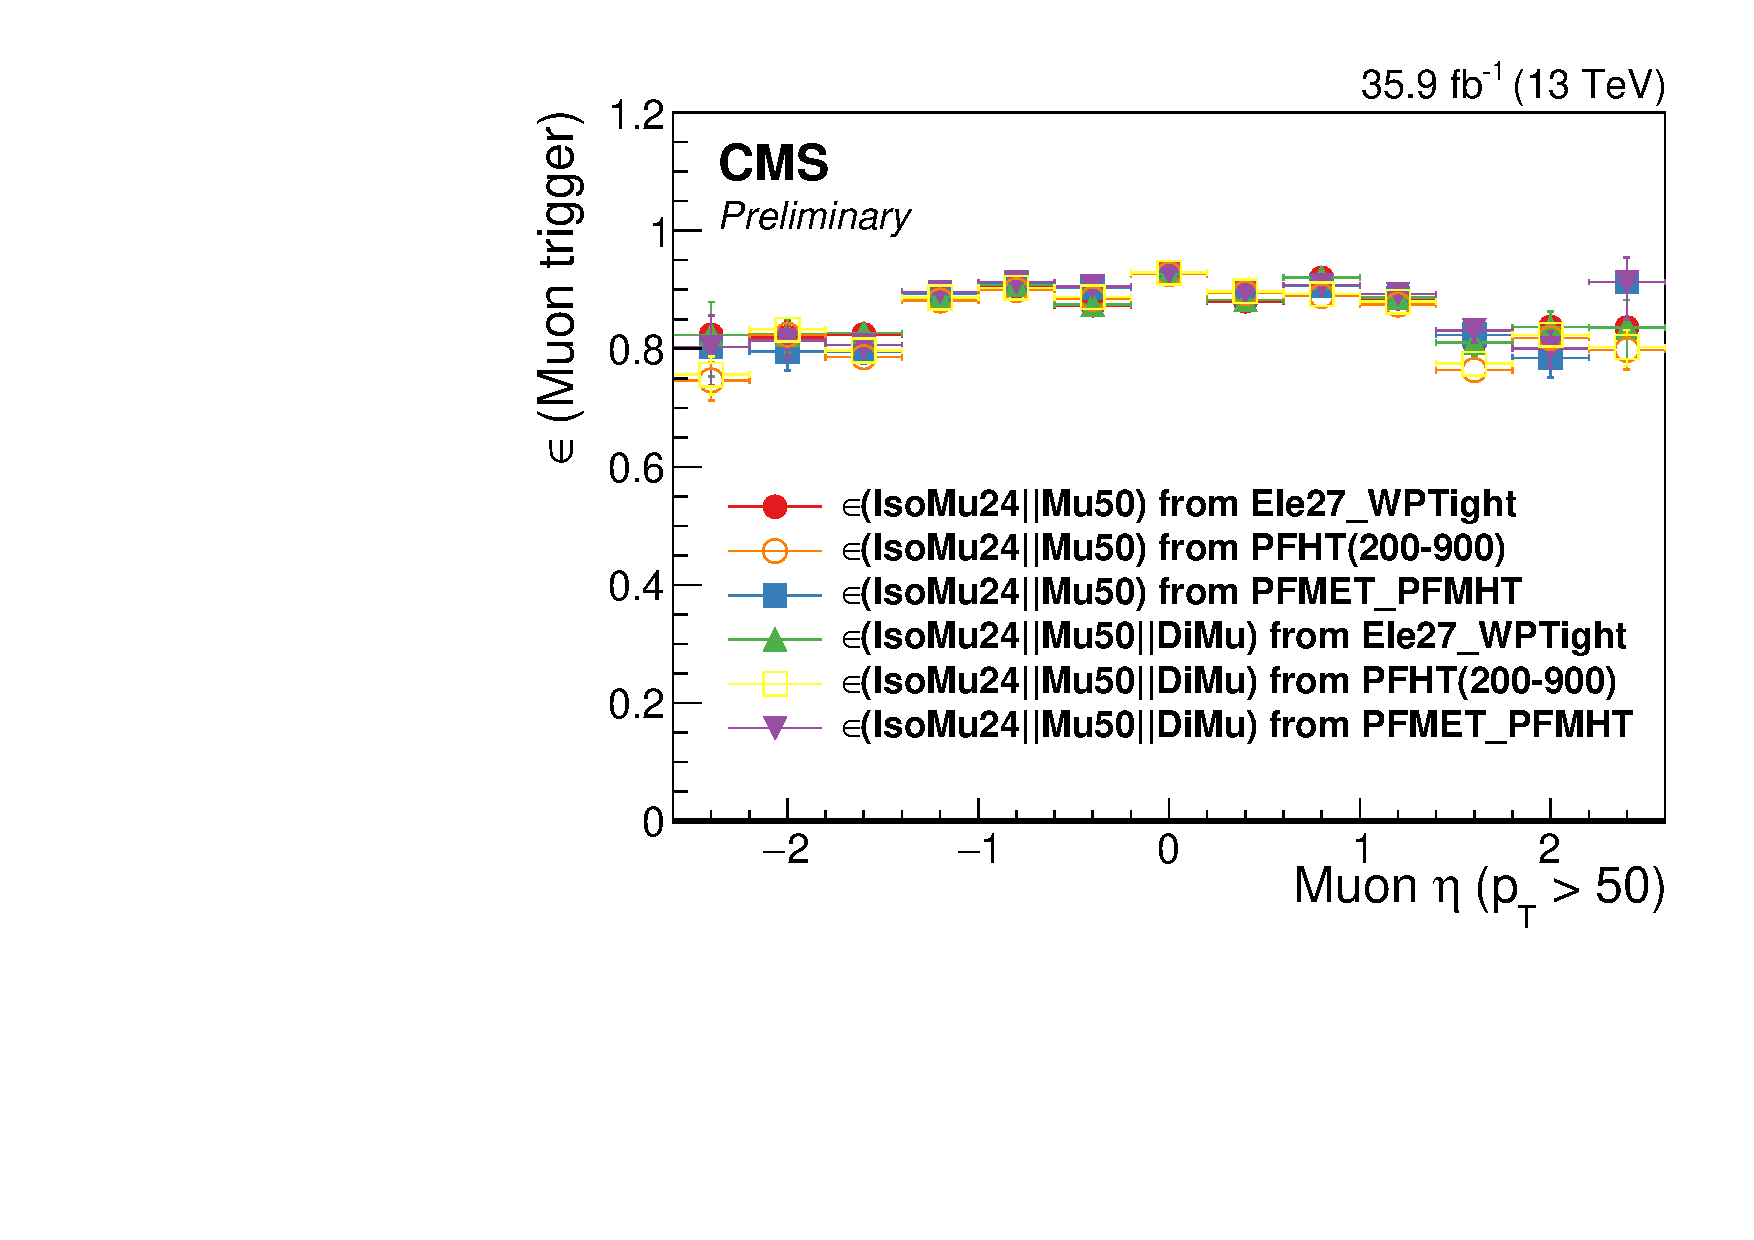
\includegraphics[width=0.49\linewidth]{sections/mc4/EvtSelSBOpt/figures/MuonEta.pdf}
   \caption{ The trigger efficiency as a function of the offline leading Muon
	 (left) $p_{T}$ and (right) $\eta$.}
   \label{fig:TrigMuon}
 \end{center}
\end{figure}

We also checked the trigger efficiency as a function of number of AK4 jets and $b$-tagged jets, after requiring the highest-$p_{T}$ muon to have $p_{T}>$ 50 GeV, as shown in Fig~\ref{fig:TrigMuonJets}. We observe similar efficiencies from the different measurements.
\begin{figure}[tbp]
 \begin{center}
   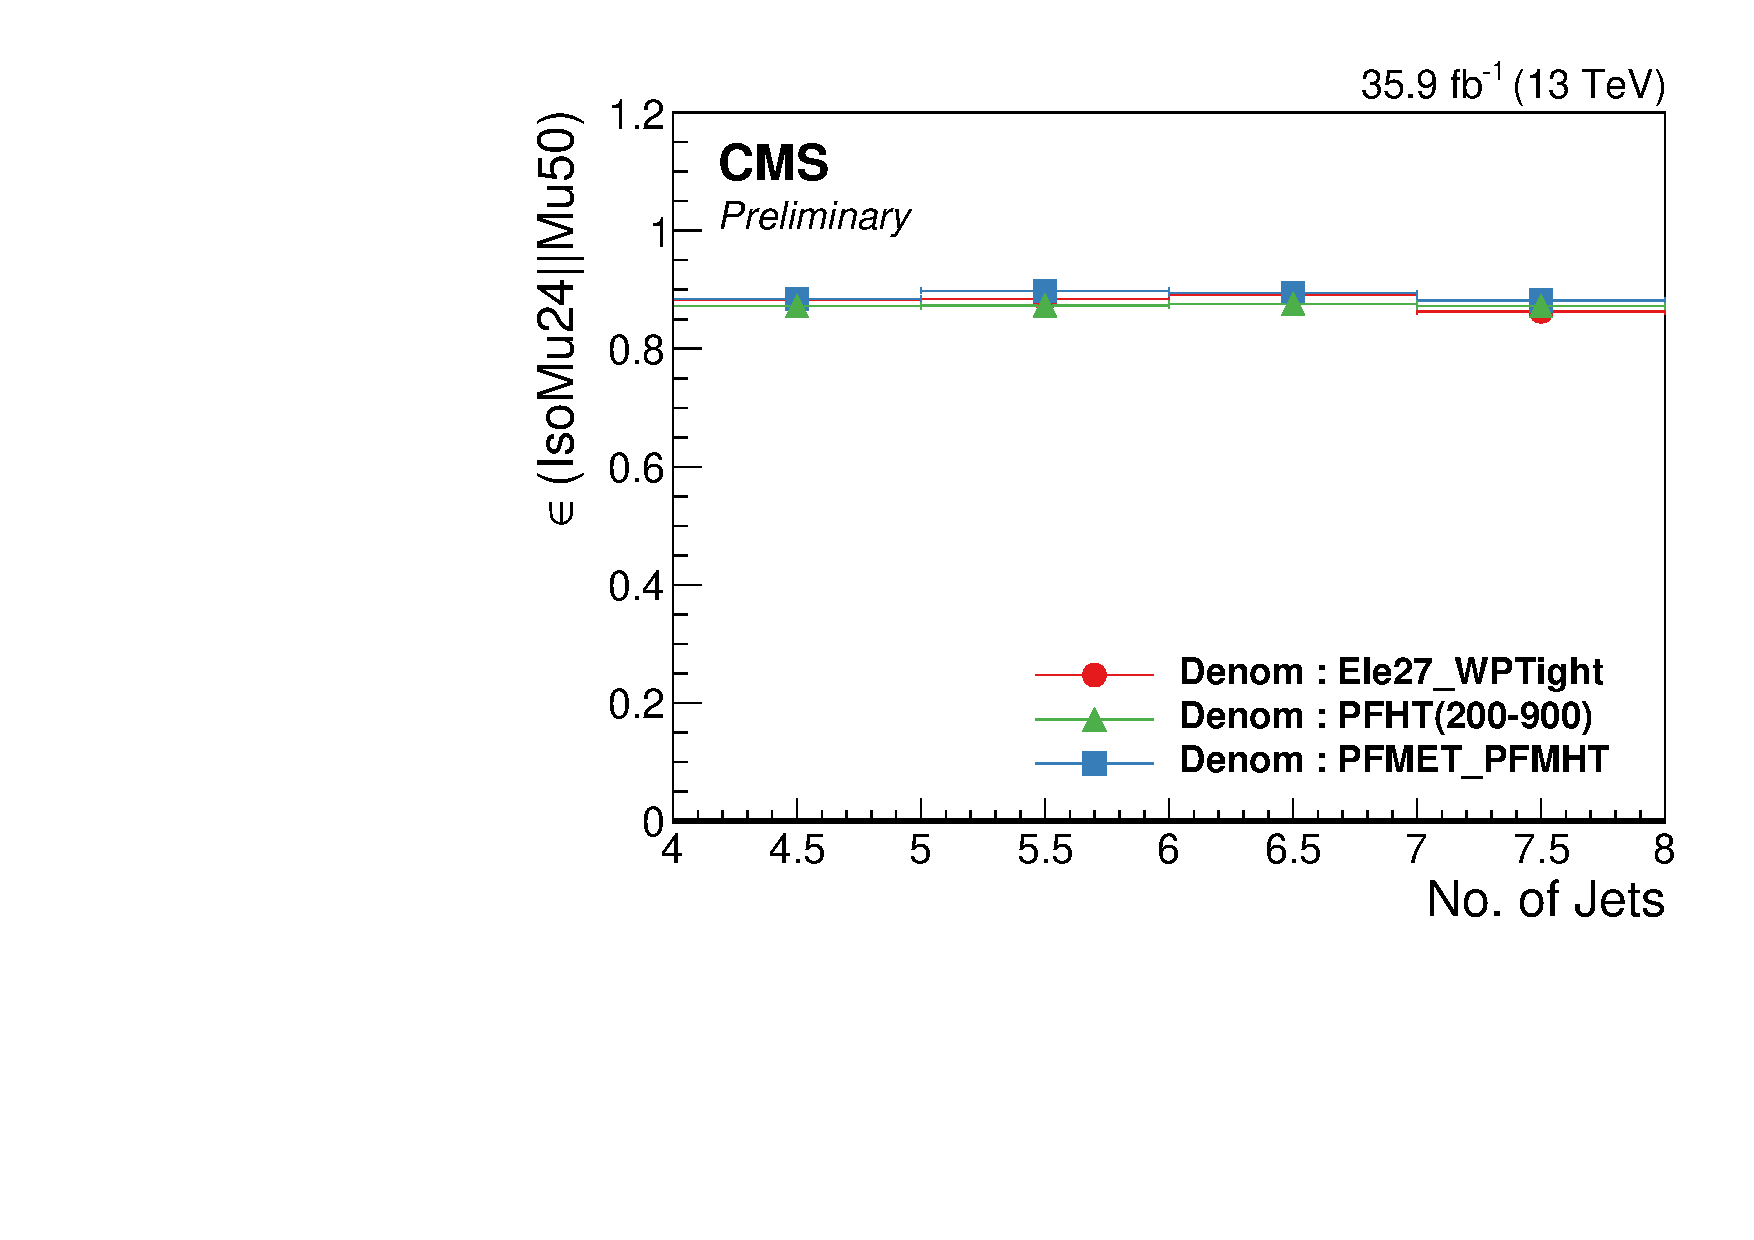
\includegraphics[width=0.49\linewidth]{sections/mc4/EvtSelSBOpt/figures/MuonNJets.pdf}
   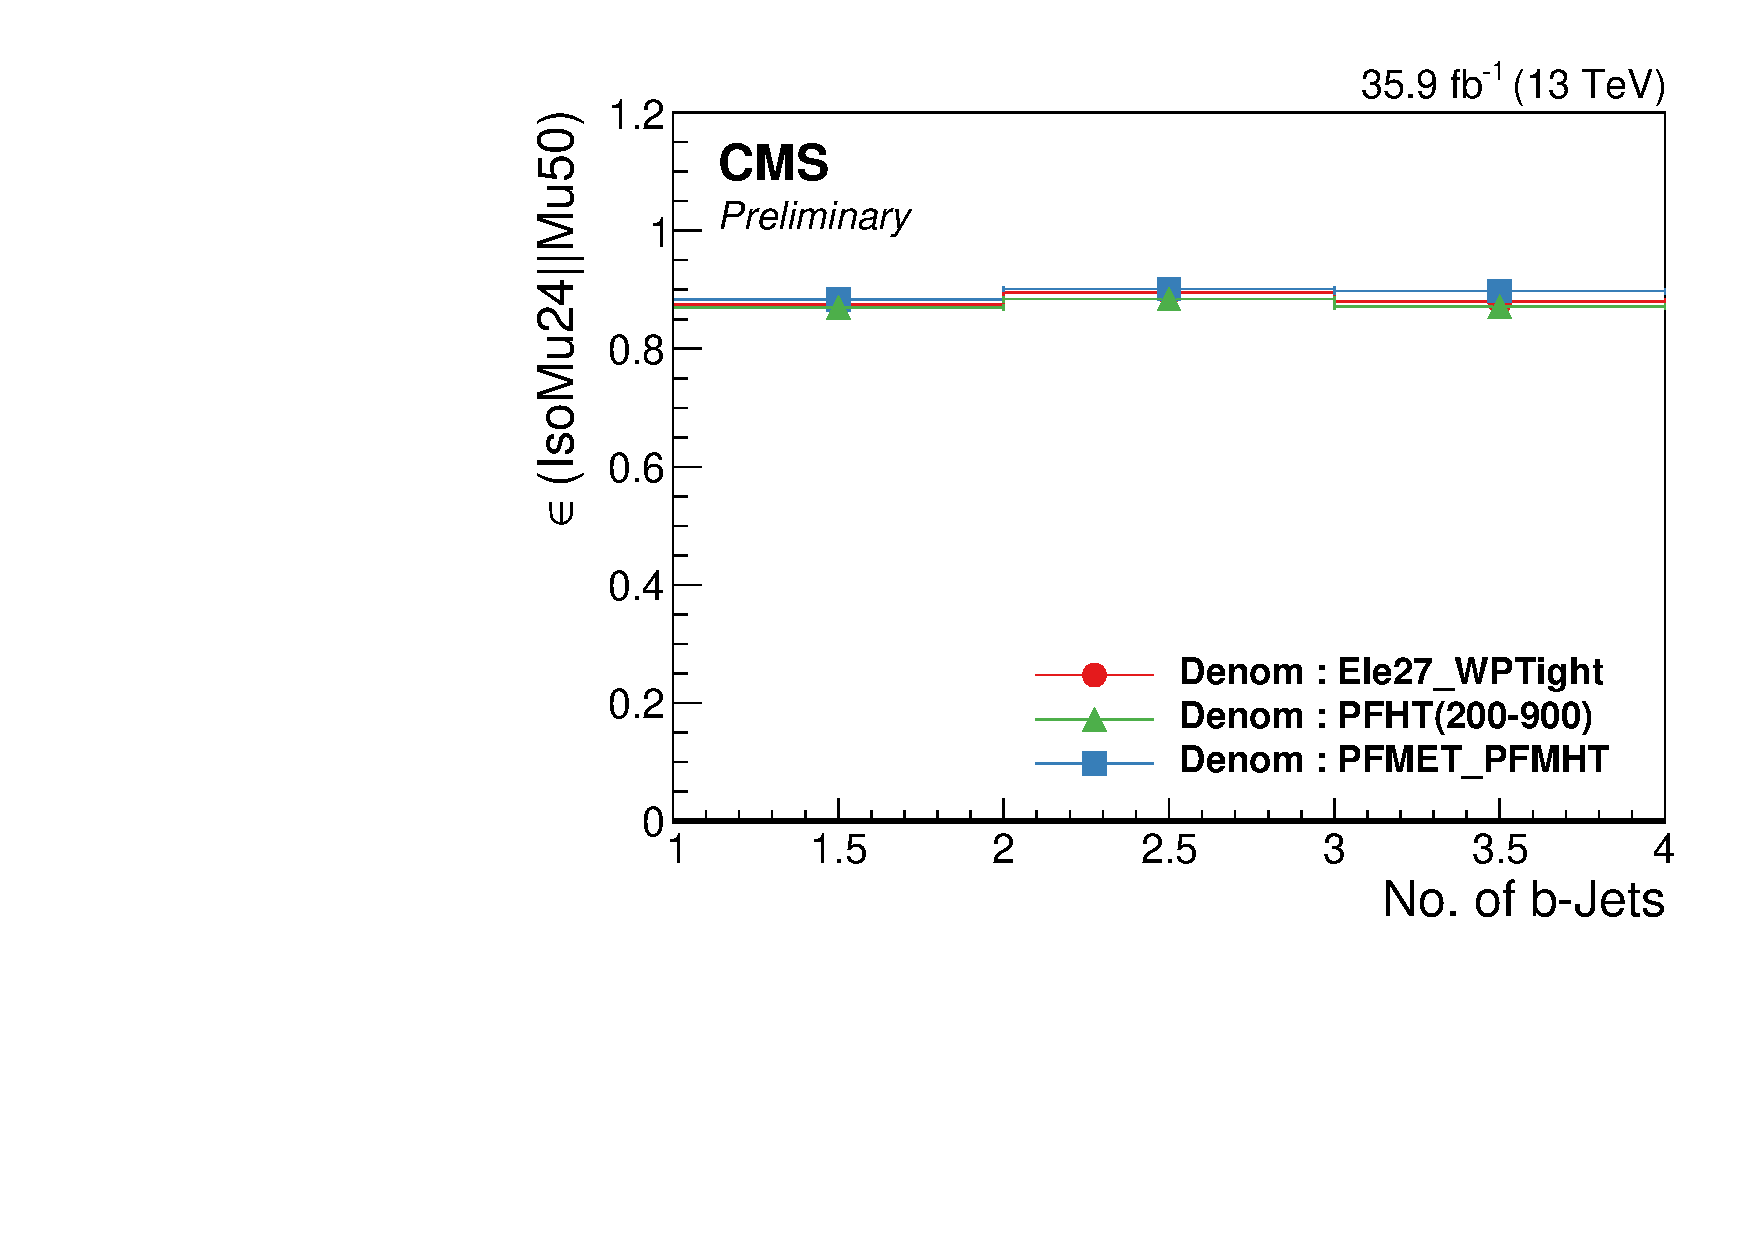
\includegraphics[width=0.49\linewidth]{sections/mc4/EvtSelSBOpt/figures/MuonNBs.pdf}
   \caption{ The trigger efficiency as a function of the offline (left) number
		 of jets with $p_{T}>$ 30 GeV and (right) number of $b$-tagged jets with $p_{T}$
		 $>$ 30GeV, with leading reconstructed muon $p_{T}$ above 50GeV from the
   single-muon trigger. The red point denote the measurement from
   single-electron dataset. The green triangle represents measurement from HT
   dataset, while blue square represents measurement from MET dataset.}
   \label{fig:TrigMuonJets}
 \end{center}
\end{figure}

\subsection{Baseline selection}
\label{sec:baselineselection}

The search is based on a sample of all-hadronic events, with b-jets decaying from top quarks, large \MET and no leptons. Initially, a loose baseline selection is applied in \MET, \HT, \njets and \nbjets. This baseline selection preserves 2-20\% of the signal events depending on the signal model. The events satisfying the baseline selection are divided into search regions defined in terms of \ntops, \nbjets, \MET, \HT and \MTTwo. By having many search regions, the analysis becomes ``inclusive", i.e., sensitive to many different signal topologies.

The following selection criteria define the baseline selection:

\begin{itemize}
\item Satisfies all filters that remove detector- and beam-related noise: 
  \begin{itemize}
    \item HBHE noise filter, 
    \item HBHEiso noise filter, 
    \item Ecal dead cell trigger primitive filter,
    \item Primary vertex filter,
    \item Bad EE super crystal filter,
    \item Global tight beam halo filter,
    \item Bad muon filter,
    \item Bad charged hadron filter,
    \item Loose JetID event filter.
  \end{itemize}

\item $\njets\geq4$:

Since the top squark is produced in pairs and each top squark decays to a top quark and an LSP, the all-hadronic final state will contain at least six jets. Not all the jets satisfy the selection criteria, therefore we only require at least four jets. Jets are reconstructed with the PF technique and clustered with the anti-$k_\mathrm{T}$ algorithm with a resolution parameter 0.4~\cite{Cacciari:2008gp} (AK4). Every jet is required to have $p_{T}>$30 GeV and $|\eta|<$2.4. In addition, they must satisfy the loose jet ID criteria for PF jets as recommended by the JetMET group. If any of the jets fail the loose jet ID criteria, the event is rejected (referred to as the loose JetID event filter above).

The two jets with highest $p_{T}$ are required to have $p_{T}>$50 GeV since SUSY predicts centrally produced jets with 
high $p_{T}$.

\item \MET $\ge$ 250 GeV, where we use the type1-corrected particle-flow \MET, with the jet energy corrections (Summer16\_23Sep2016V3). The selection threshold is constrained by trigger efficiency requirements.

\item \MTTwo $\ge$ 200 GeV, which is mainly used to reduce SM background events with low value of \MTTwo. The \MTTwo variable works especially well for the \ttbar events, where the \MTTwo shows a kinematic edge around the top quark mass.

\item \HT $\ge$ 300 GeV, with \HT = $\sum_{\mathrm{jets}} p_{T}$, the scalar $p_{T}$ sum over jets. Jets in the \HT calculation must meet the same jet selection criteria defined above.

\item \nbjets $\ge$ 1, with b-jets identified using the CSV b-tagging algorithm (CSVM), medium working point.

\item Muon veto:

Muon candidates are selected using the ``Medium Muon" selection, recommended by the muon Physics Objects Group (POG). Muon candidates must satisfy $p_{T}>10$ GeV and $|\eta|<2.4$. Details of the muon medium ID criteria are listed in the Table~\ref{tab:MuonMediumID} and Table~\ref{tab:MuonMediumIDGoodGlobalMuon}. In addition to the official medium selection, we also apply an impact parameter requirement, with details listed in Table~\ref{tab:MuonMediumIDImpactParameter}. A PF relative-isolation criteria is applied (mini-isolation), for which the isolation cone shrinks as a function of increasing muon $p_{T}$. The $p_{T}$ in the mini-isolation cone is required to be less than 20\% of the muon $p_{T}$ to eliminate events with an isolated muon. 

\newsavebox{\closureBox}

\begin{table}[htbp]
\fontsize{10 pt}{1.2 em}
\selectfont
\begin{centering}
\caption{\label{tab:MuonMediumID} Muon Medium ID 2016 HIP Safe.}
\hspace*{-4ex}
\begin{lrbox}{\closureBox}
\begin{tabular}{|c|c|}
\hline
  Muon Medium ID                                      &               \\
\hline
  Loose muon ID                                       & Yes           \\
\hline
  Fraction of valid tracker hits $>$                  & 0.80          \\
\hline
  Good Global muon OR Tight segment compatibility $>$ & Yes OR 0.451 \\
\hline
\end{tabular}
\end{lrbox}
\scalebox{0.80}{\usebox{\closureBox}}
\par\end{centering}
\end{table}

\begin{table}[htbp]
\fontsize{10 pt}{1.2 em}
\selectfont
\begin{centering}
\caption{\label{tab:MuonMediumIDGoodGlobalMuon} Muon Medium ID HIP Safe Good Global Muon.}
\hspace*{-4ex}
\begin{lrbox}{\closureBox}
\begin{tabular}{|c|c|}
\hline
  Good Global muon                      &       \\
\hline
  Global muon                           & Yes   \\
\hline
  Normalized global-track $\chi^{2} <$  & 3     \\
\hline
  Tracker-Standalone position match $<$ & 12    \\
\hline
  Kick finder $<$                       & 20    \\
\hline
  Segment compatibility $>$             & 0.303 \\
\hline
\end{tabular}
\end{lrbox}
\scalebox{0.80}{\usebox{\closureBox}}
\par\end{centering}
\end{table}

\begin{table}[htbp]
\fontsize{10 pt}{1.2 em}
\selectfont
\begin{centering}
\caption{\label{tab:MuonMediumIDImpactParameter} Additional Impact Parameter cut on Muon.}
\hspace*{-4ex}
\begin{lrbox}{\closureBox}
\begin{tabular}{|c|c|}
\hline
  Muon Impact Parameter &     \\
\hline
  d0 $<$                & 0.2 \\
\hline
  dz $<$                & 0.5 \\
\hline
\end{tabular}
\end{lrbox}
\scalebox{0.80}{\usebox{\closureBox}}
\par\end{centering}
\end{table}

\item Electron veto:

Electron candidates are selected using the POG-recommended ``Cut Based VETO" selection. Different selection criteria are applied to the barrel and endcap electromagnetic calorimeter regions. The selection criteria are listed in Table~\ref{tab:ElectronCutBasedVeto}. 

Electrons are required to have $p_{T}>10$ GeV and $|\eta|<2.5$. Reconstructed isolated electrons are rejected using PF-based ``mini-isolation" criteria, requiring less than 10\% of the electron energy in the isolation cone.

\begin{table}[htbp]
\fontsize{10 pt}{1.2 em}
\selectfont
\begin{centering}
\caption{\label{tab:ElectronCutBasedVeto} Electron Cut Based Veto 2016 Data in 80X CMSSW offline reconstruction condition.}
\hspace*{-4ex}
\begin{lrbox}{\closureBox}
\begin{tabular}{|c|c|c|}
\hline
                                     & ECAL Barrel($|Eta|<1.479$) & ECAL Endcap($|Eta|>1.479$) \\
\hline
  full5x5 sigmaIetaIeta $<$          & 0.0115                     & 0.037                    \\
\hline
  abs(dEtaInSeed) $<$                & 0.00749                    & 0.00895                  \\
\hline
  abs(dPhiIn) $<$	             & 0.228                      & 0.213                    \\
\hline
  H/E $<$	                     & 0.356                      & 0.211                    \\
\hline
  Rel. comb. PF iso with EA corr $<$ & 0.175                      & 0.159                    \\
\hline
  abs(1/E-1/p) $<$                   & 0.299                      & 0.15                     \\
\hline
  expected missing inner hits $<$    & 3                          & 4                        \\
\hline
  pass conversion veto               & yes                        & yes                      \\
\hline
\end{tabular}
\end{lrbox}
\scalebox{0.80}{\usebox{\closureBox}}
\par\end{centering}
\end{table}

\item Angular criteria:

Selection criteria on the angles between \MET and the three jets with highest $p_{T}$, $\Delta\phi(\MET, j_{1,2,3})>$ 0.5, 0.5, 0.3, are applied to remove events arising from QCD processes.

\item Isolated track veto:

After applying the criteria described above, the residual background comes from \ttbar, single top, and $W+$jets events with one $W\rightarrow l\nu$
decay where $l$ can be an electron or muon that is not identified, or a hadron from single-prong hadronic $\tau$ lepton decay. To further suppress these backgrounds, we reject events 
that have one or more isolated tracks. The track isolation
is calculated from charged PF candidates consistent with the 
reconstructed primary vertex ($|dz(PV)|<0.1~\mathrm{cm}$).
The requirements are different for muon, electron and charged hadron tracks.
For both electron and muon tracks, the isolated track requirements are: 
$p_{T}>$5 GeV, $|\eta|<$2.5 and relative isolation less than 0.2.
For charged hadron tracks, the $p_{T}$ requirement
is raised to be at least 10 GeV and the relative isolation value to be less 
than 0.1. To retain more signal, and thus improve signal-to-background
event discrimination, events with one isolated track, as defined
above, are rejected only if they satisfy
  \begin{equation}
    \label{eq:mt_isotk}
    m_T(tk,\MET) = \sqrt{2p_{T}^{tk}\MET(1-\cos\Delta\phi)}<100\;\mathrm{GeV}
  \end{equation}
  where $p_{T}^{tk}$ is the transverse momentum of the track and
  $\Delta\phi$ is the azimuthal separation between the track and \MET
  vector. 

\end{itemize}

\subsection{Search regions}
\label{sec:searchregions}

In the analysis of the 2016 data, we bin the search regions in terms of the number of b-tagged jets and top quark candidates. 
The top quark reconstruction and identification procedure (top-tagging) is described in Sec.~\ref{sec:toptagger}. 

In order to improve background suppression, in particular the \ttbar
contribution, the \MET, \HT and \MTTwo variables were added to the 
set that defines the search regions. The variable 
\MTTwo~\cite{Lester:1999tx,Barr:2003rg} is an extension of the transverse 
mass variable that is sensitive to the pair production of heavy particles, each
of which decays to a visible particle and an invisible particle.
The \pTop, the \pRsystem, and the \MET in an event
are used to construct \MTTwo assuming the invisible particles are massless.
In order to illustrate how \MTTwo is calculated, let us take the process 
${\rm pp} \rightarrow \sTop\santiTop\rightarrow t\bar{t}\chi_1^0\chi_1^0$
as an example. This process contains two simultaneous decays of an unseen 
particle of unknown mass(\sTop or \santiTop) into an invisible 
particle ($\chi_1^0$) and visible particle ($t$ or $\bar{t}$). The
variable \MTTwo is defined as:
\begin{equation} \label{eq:MT2}
   \begin{array}{l}
     \displaystyle{ \MTTwo \equiv \min_{\vec{q}_{T}^{(1)}+\vec{q}_{T}^{(2)} = \vec{p}_{T}} [\max\{m_{T}^2(\vec{p}_{T}^{t^{(1)}}, \vec{q}_{T}^{(1)}; m_{\chi_1^0}), m_{T}^2(\vec{p}_{T}^{t^{(2)}}, \vec{q}_{T}^{(2)}; m_{\chi_1^0})\}]  } 
   \end{array}
\end{equation}
where the $m_{T}^2$ is the transverse mass,
\begin{equation} \label{eq:MTdef}
   \begin{array}{l}
     \displaystyle{
        m_{T}^2(\vec{p}_{T}^{t^{(1)}}, \vec{q}_{T}^{(1)}; m_{\chi_1^0}) \equiv m_{t^{(1)}}^{2} + m_{\chi_1^0}^2 + 2(E_{T}^{t^{(1)}}E_{T}^{(1)} - \vec{p}_{T}^{t^{(1)}} \cdot \vec{q}_{T}^{(1)})
     }
   \end{array}
\end{equation} 

\MTTwo is a minimization of two transverse masses with a constraint that 
the sum of the transverse momenta of both $\chi_1^0$'s be equal to the 
missing transverse momentum in the event, i.e., $\vec{q}_{T}^{(1)}+\vec{q}_{T}^{(2)} = \vec{p}_{T}$. 
\MTTwo has a kinematic upper limit at the \sTop mass. 
The superscripts $(1)$ and $(2)$ in the equations refer to the individual 
decays of the \sTop particles. In the specific case of the analysis described
in this thesis, we replace the quantities related to superscript $(1)$ by those
of associated with the fully reconstructed top quark, i.e., the \pTop. 
Similarly, we replace the quantities related to superscript $(2)$ by those
of the partially reconstructed top quark, i.e., the \pRsystem 
for $\ntops =1$ and the fully reconstructed top quark for $\ntops \ge 2$. 
\MET then corresponds to $\vec{p}_{T}$ in the equation~\ref{eq:MT2}. 
Since we assume that the invisible particle is massless, $m_{\chi_1^0}$ is set to zero in Eqs.~\ref{eq:MT2}-~\ref{eq:MTdef}. 

Briefly, we start from the fact that at least one hadronic top quark candidate is required to be present in the search sample. 
If there are two top quark candidates, \MTTwo is calculated using the pair of top 
candidates and \MET. In case there are more than two top candidates
in the sample, we compute \MTTwo for all combinations and choose the 
\MTTwo with the smallest value. If there is only one top quark candidate identified
by the top-tagging algorithm, we reconstruct the other top 
quark from the remanent of the event using the b-tagged jet (or the hardest $p_{T}$ jet if no b-tagged jet found) as a seed and the R-sys 
jet closest to the seed jet with an invariant mass between 50 GeV and 
the nominal top quark mass. In case no combination satisfies the invariant mass
requirement, we use the seed jet as the only remanent of the other 
top quark. In the latter case, \MTTwo is calculated from the reconstructed top candidate, the remanent and the \MET.

Figs~\ref{fig:compSBvars1} and \ref{fig:compSBvars2} show a comparison between total SM backgrounds from simulation and several signal points for the four search bin variables after the baseline selection requirements. We can clearly see that all the variables have good discrimination power. The data are also shown and the total SM backgrounds are scaled to the same yield as the data.

\begin{figure}[h]
  \begin{center}
    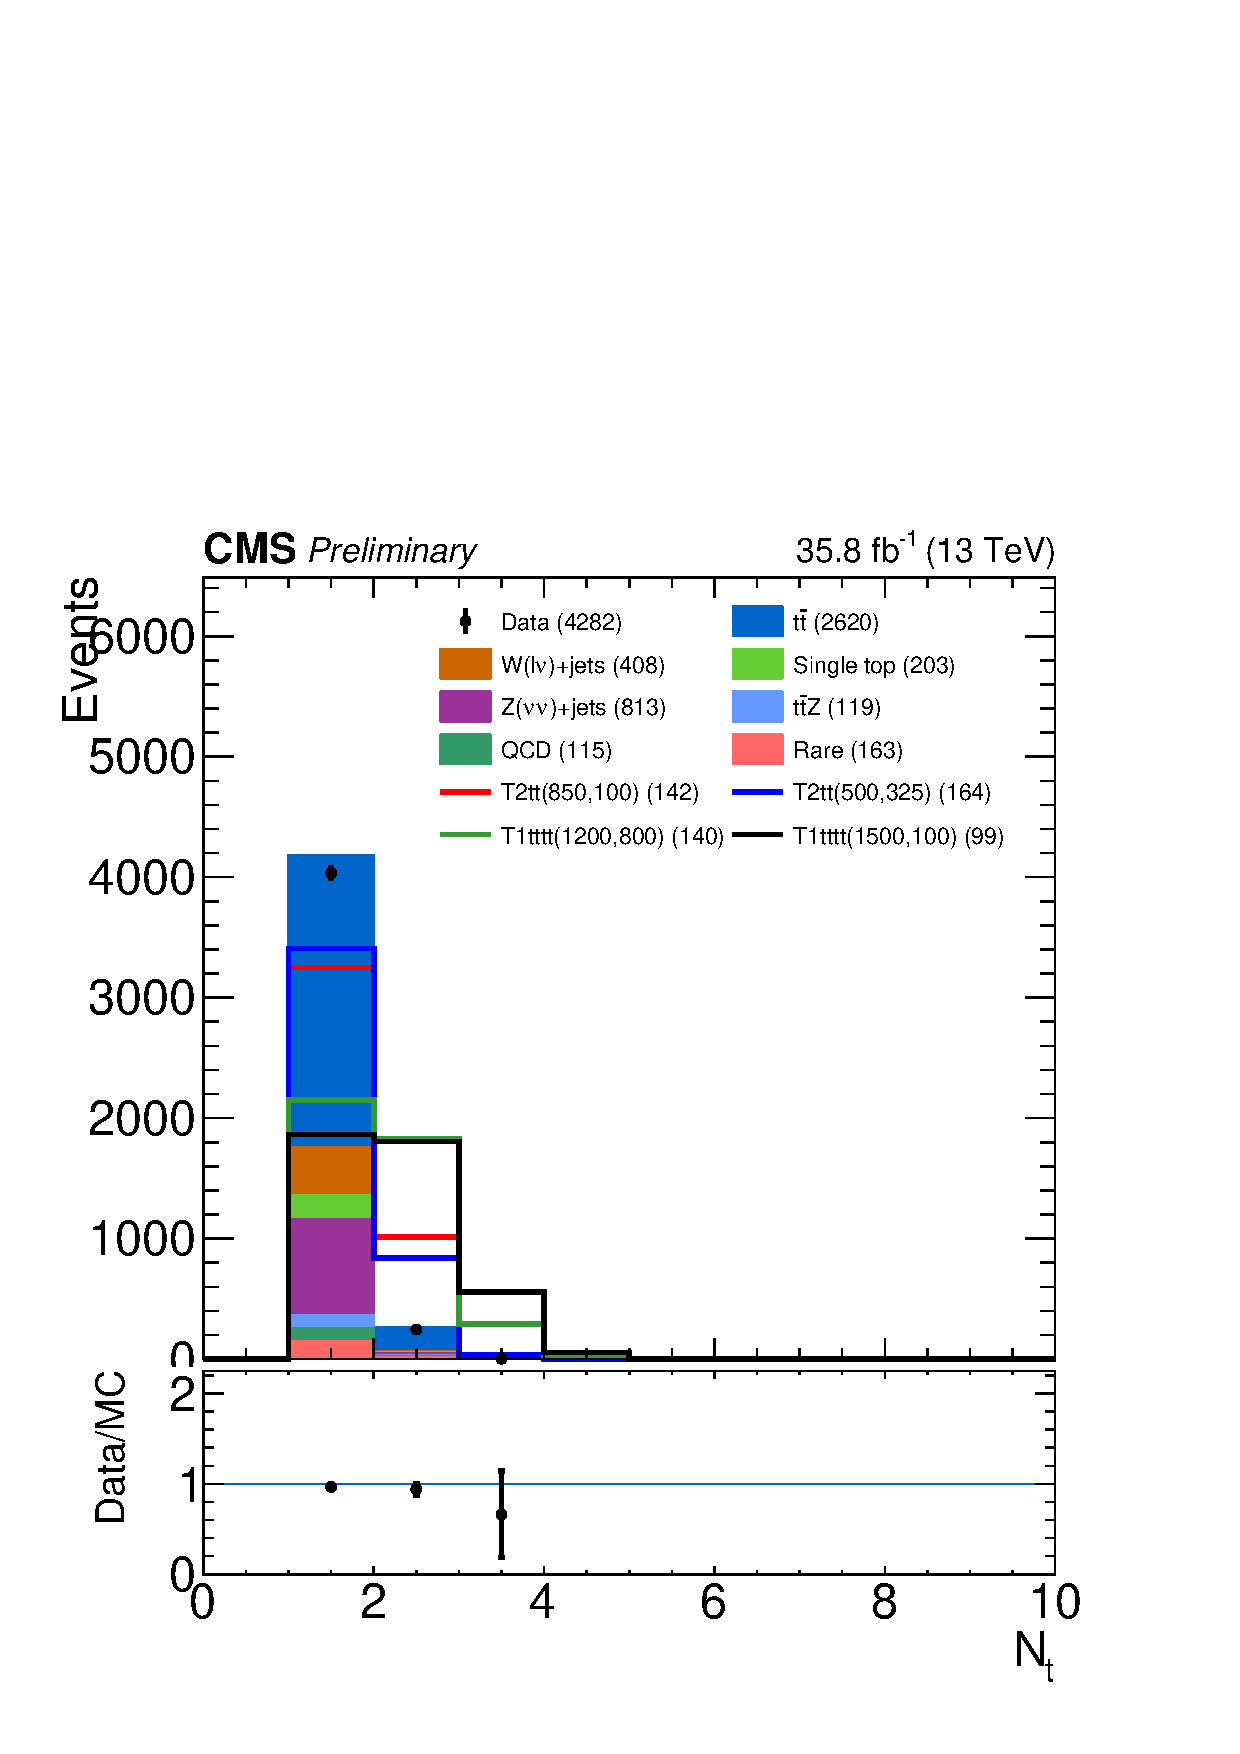
\includegraphics[width=0.45\linewidth]{sections/mc4/EvtSelSBOpt/figures/DataMC_MET_model_NTops_baseline.pdf}
    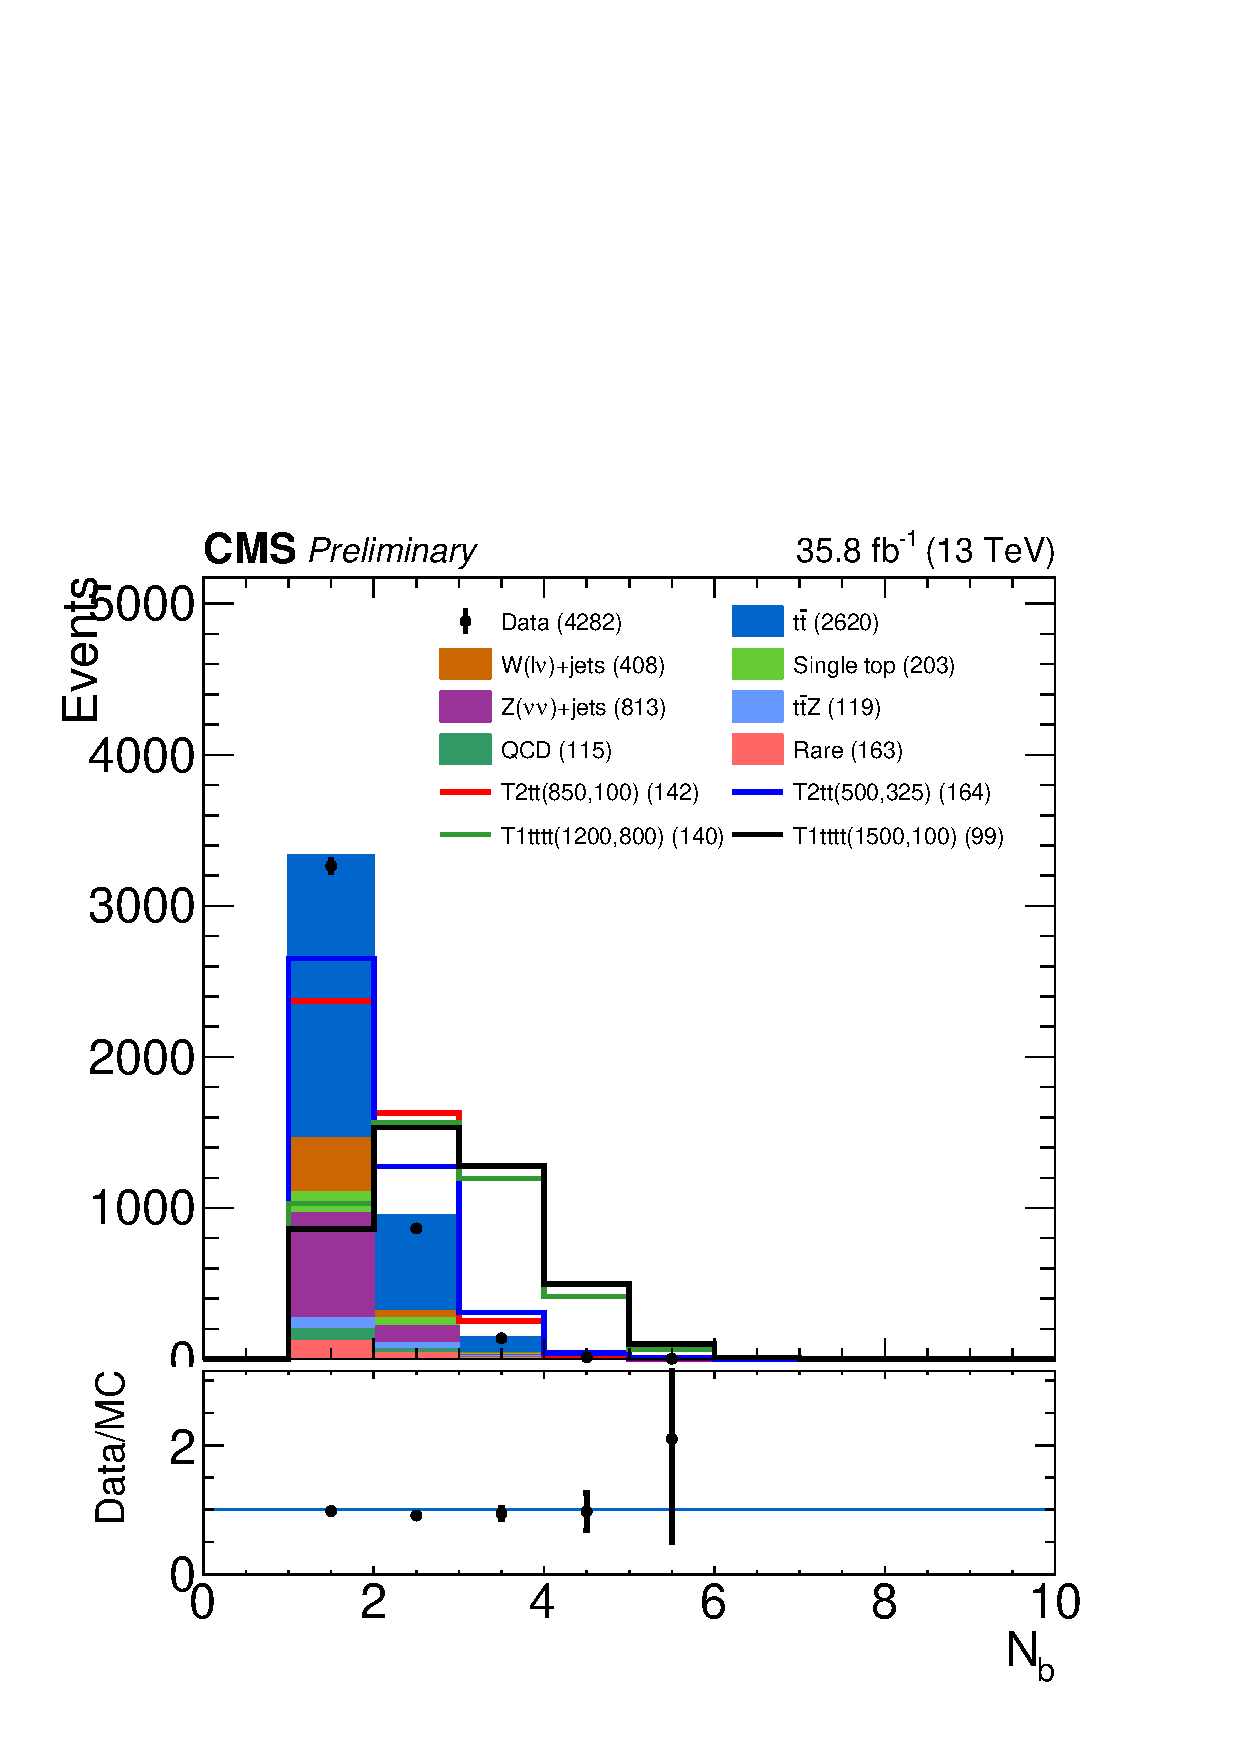
\includegraphics[width=0.45\linewidth]{sections/mc4/EvtSelSBOpt/figures/DataMC_MET_model_NBJEts_baseline.pdf}\\
    \caption{Comparison of the distributions between total SM backgrounds from simulation and several signal points for \ntops at the left and \nbjets at the right. Total SM backgrounds and signals are scaled to same data yield for a shape comparison. The yields for the Data and the SM backgrounds are in the legend.  The scale is included in the legend for the signal points. }
    \label{fig:compSBvars1}
  \end{center}
\end{figure}

\begin{figure}[h]
  \begin{center}
    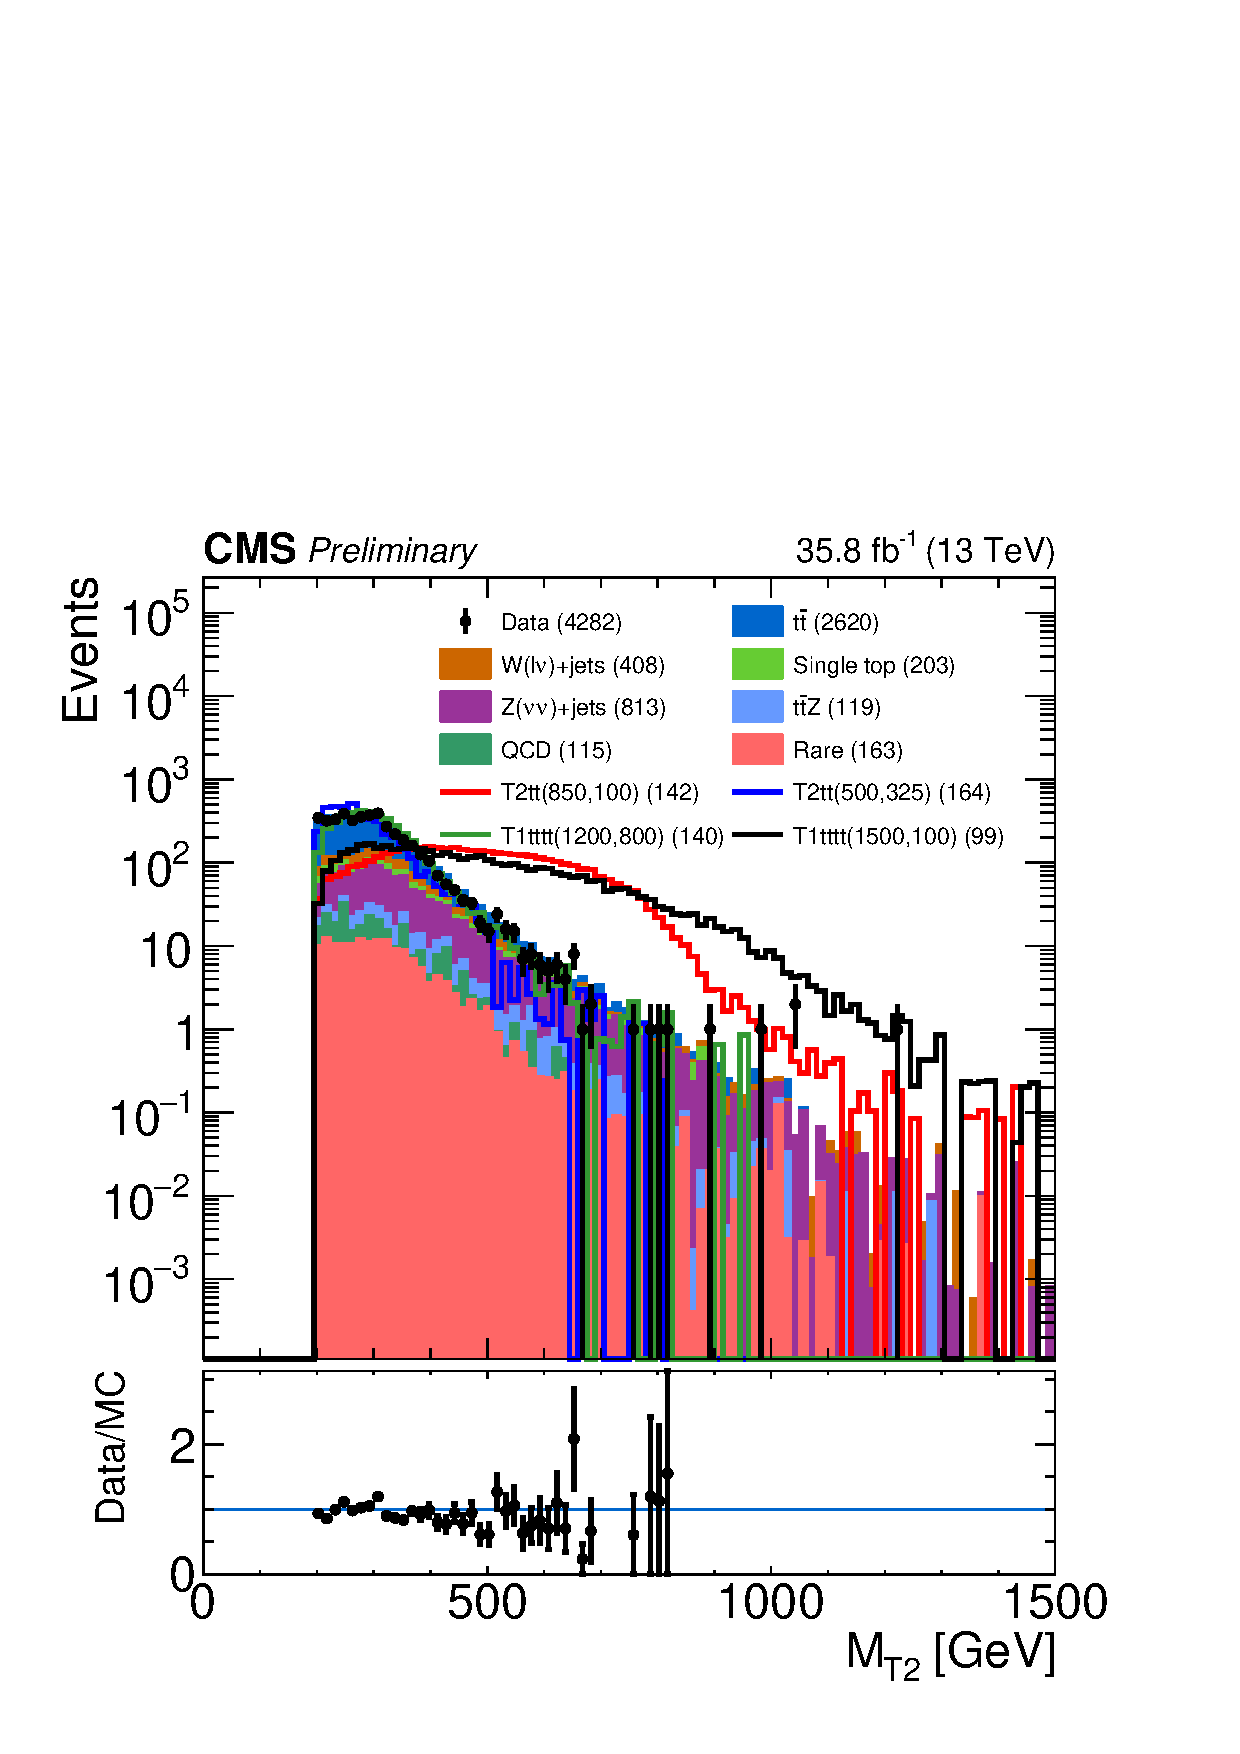
\includegraphics[width=0.45\linewidth]{sections/mc4/EvtSelSBOpt/figures/DataMC_MET_model_MT2_baseline.pdf}
    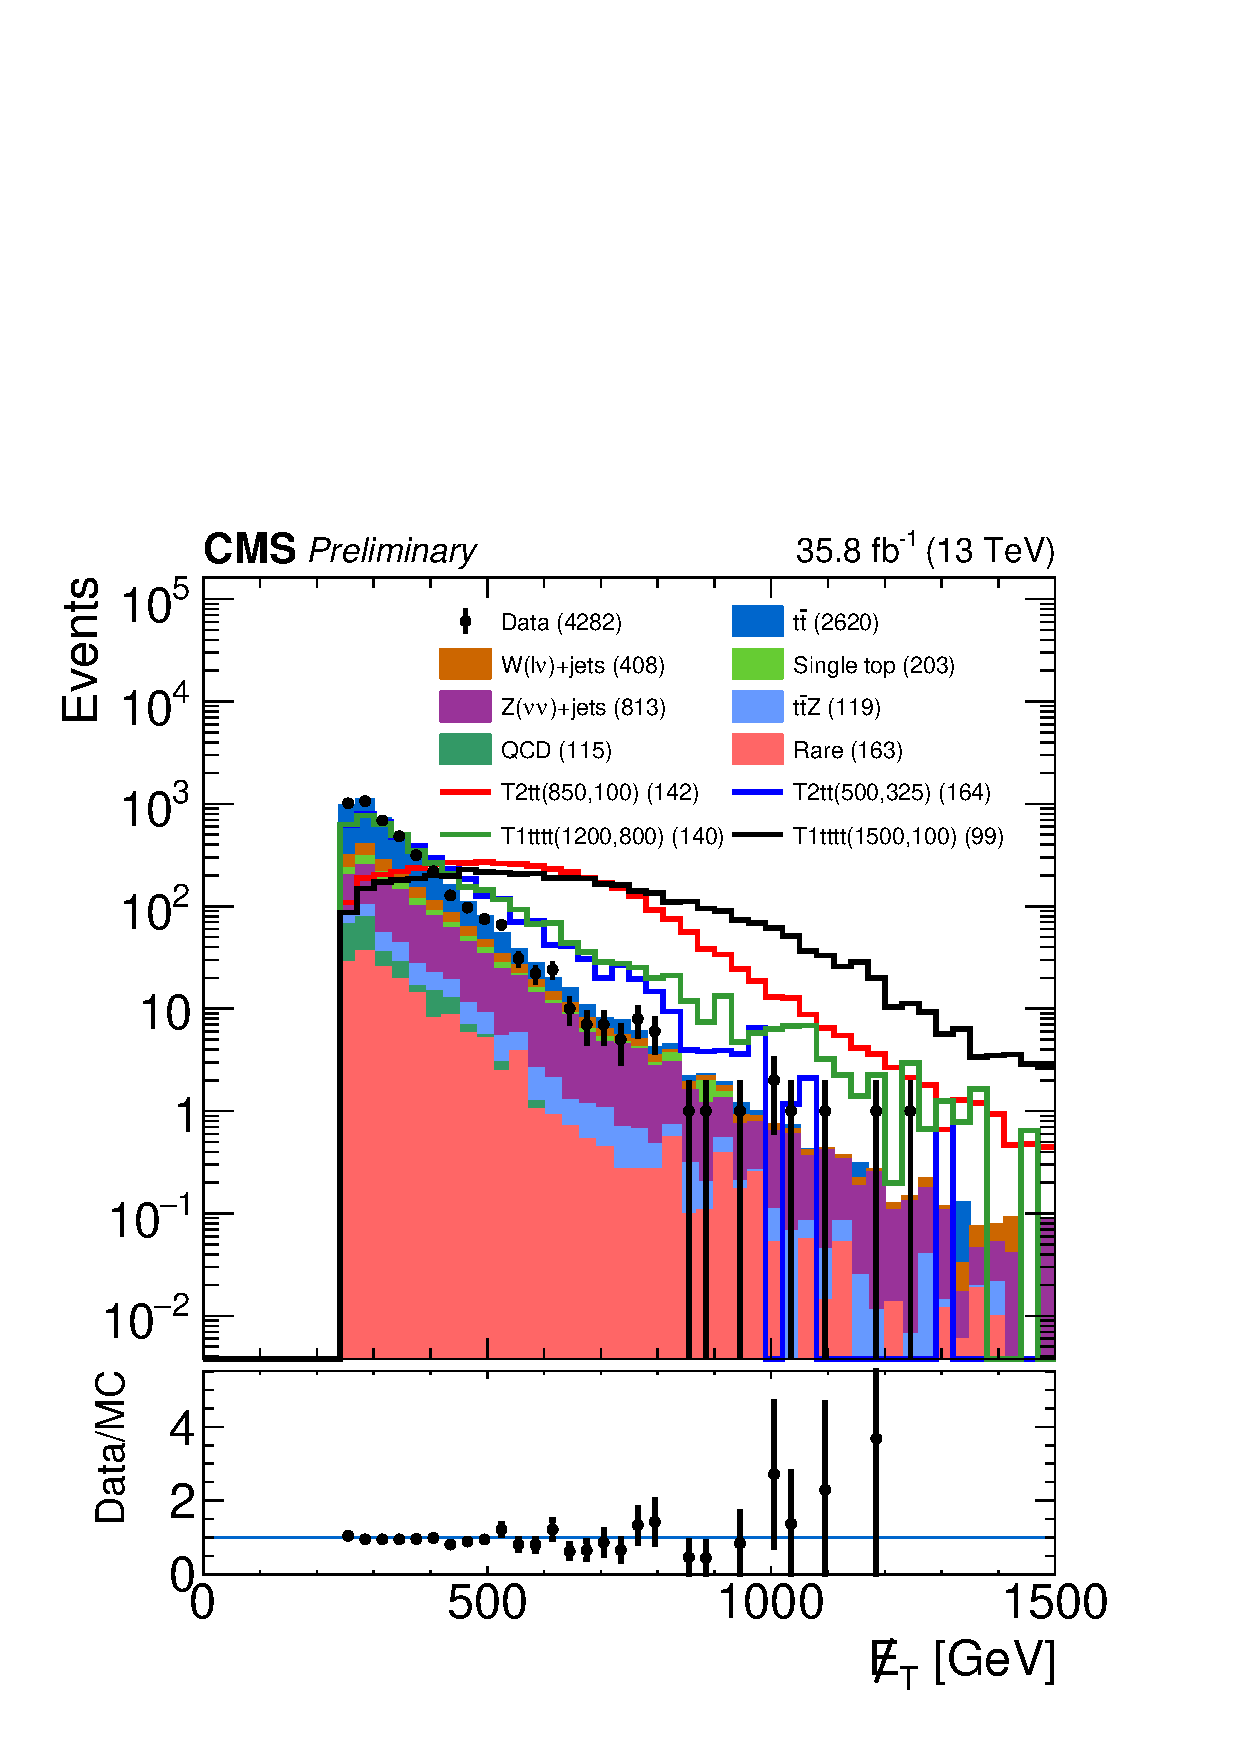
\includegraphics[width=0.45\linewidth]{sections/mc4/EvtSelSBOpt/figures/DataMC_MET_model_met_baseline.pdf}
    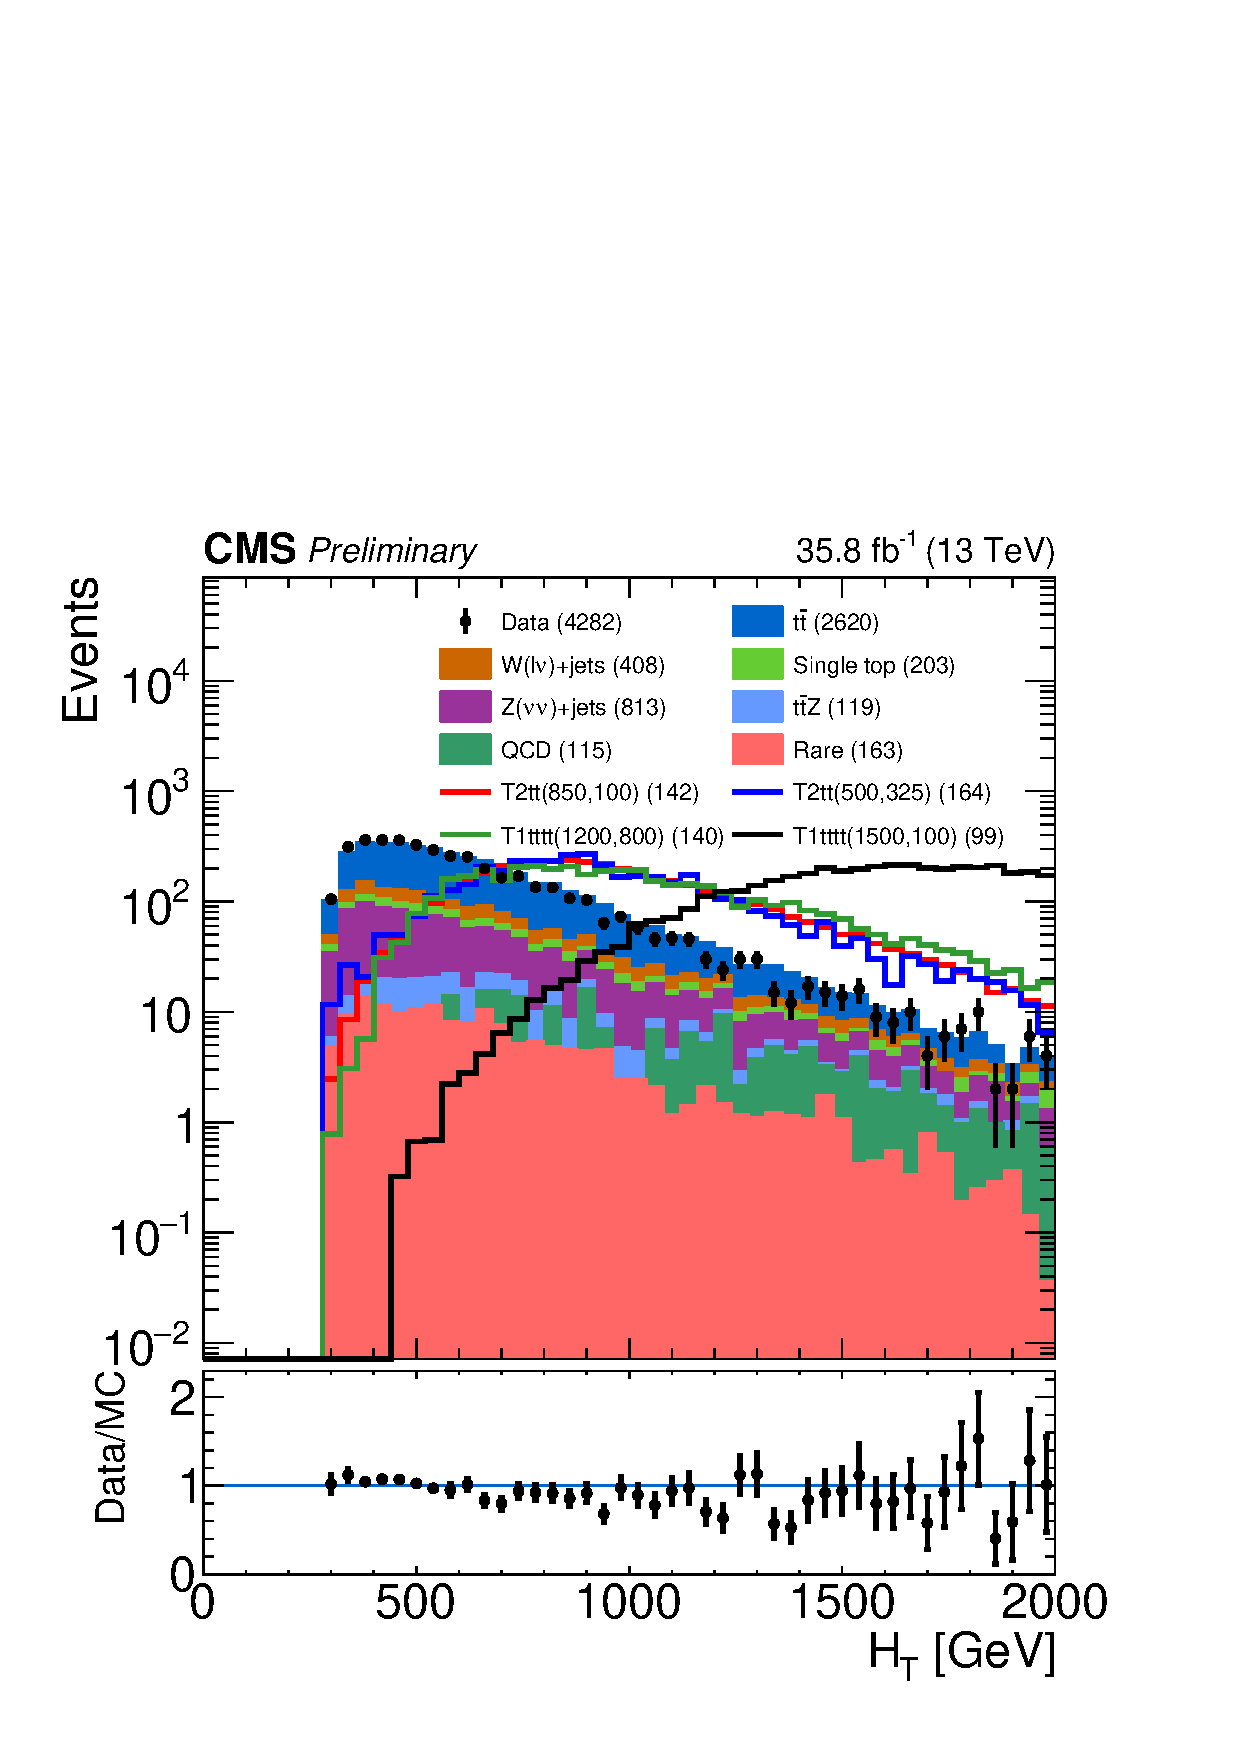
\includegraphics[width=0.45\linewidth]{sections/mc4/EvtSelSBOpt/figures/DataMC_MET_model_ht_baseline.pdf}\\
    \caption{Comparison of the distributions between total SM backgrounds from simulation and several signal points for \MET at the top left and \MTTwo at the top right with \HT at the bottom. Total SM backgrounds and signals are scaled to same data yield for a shape comparison. The yields for the Data and the SM backgrounds are in the legend.  The scale is included in the legend for the signal points. }
    \label{fig:compSBvars2}
  \end{center}
\end{figure}

The search bins defined after the baseline selection criteria (in total 84 bins) are illustrated in Fig~\ref{fig:SBXX}. An improvement in the selection efficiency is made by switching from the \MTTwo variable to \HT variable for search bins with $\nbjets>=3$ or $\ntops>=3$ since these bins should be sensitive to the T1tttt signals where \MTTwo cannot be as clearly defined as for T2tt events.
To accommodate the larger data sample collected in 2016 compared to 2015, and improve the search sensitivity, we use a finer segmentation of the search bins in
\MET, \HT and \MTTwo than for the analysis of the 2015 data. The search bin optimization is based on a significance scan of each of \MET, \MTTwo and \HT dimension. However
further adjustment was performed to have a reasonable number of control sample events for the major background predictions.
The numbers displayed in the figures are the binning indices that are used throughout the analysis.
The bins with $\ntops>=3$ are important for T1tttt signal but for T2tt we do not use them for the limit calculation.

\begin{figure}[h]
  \begin{center}
    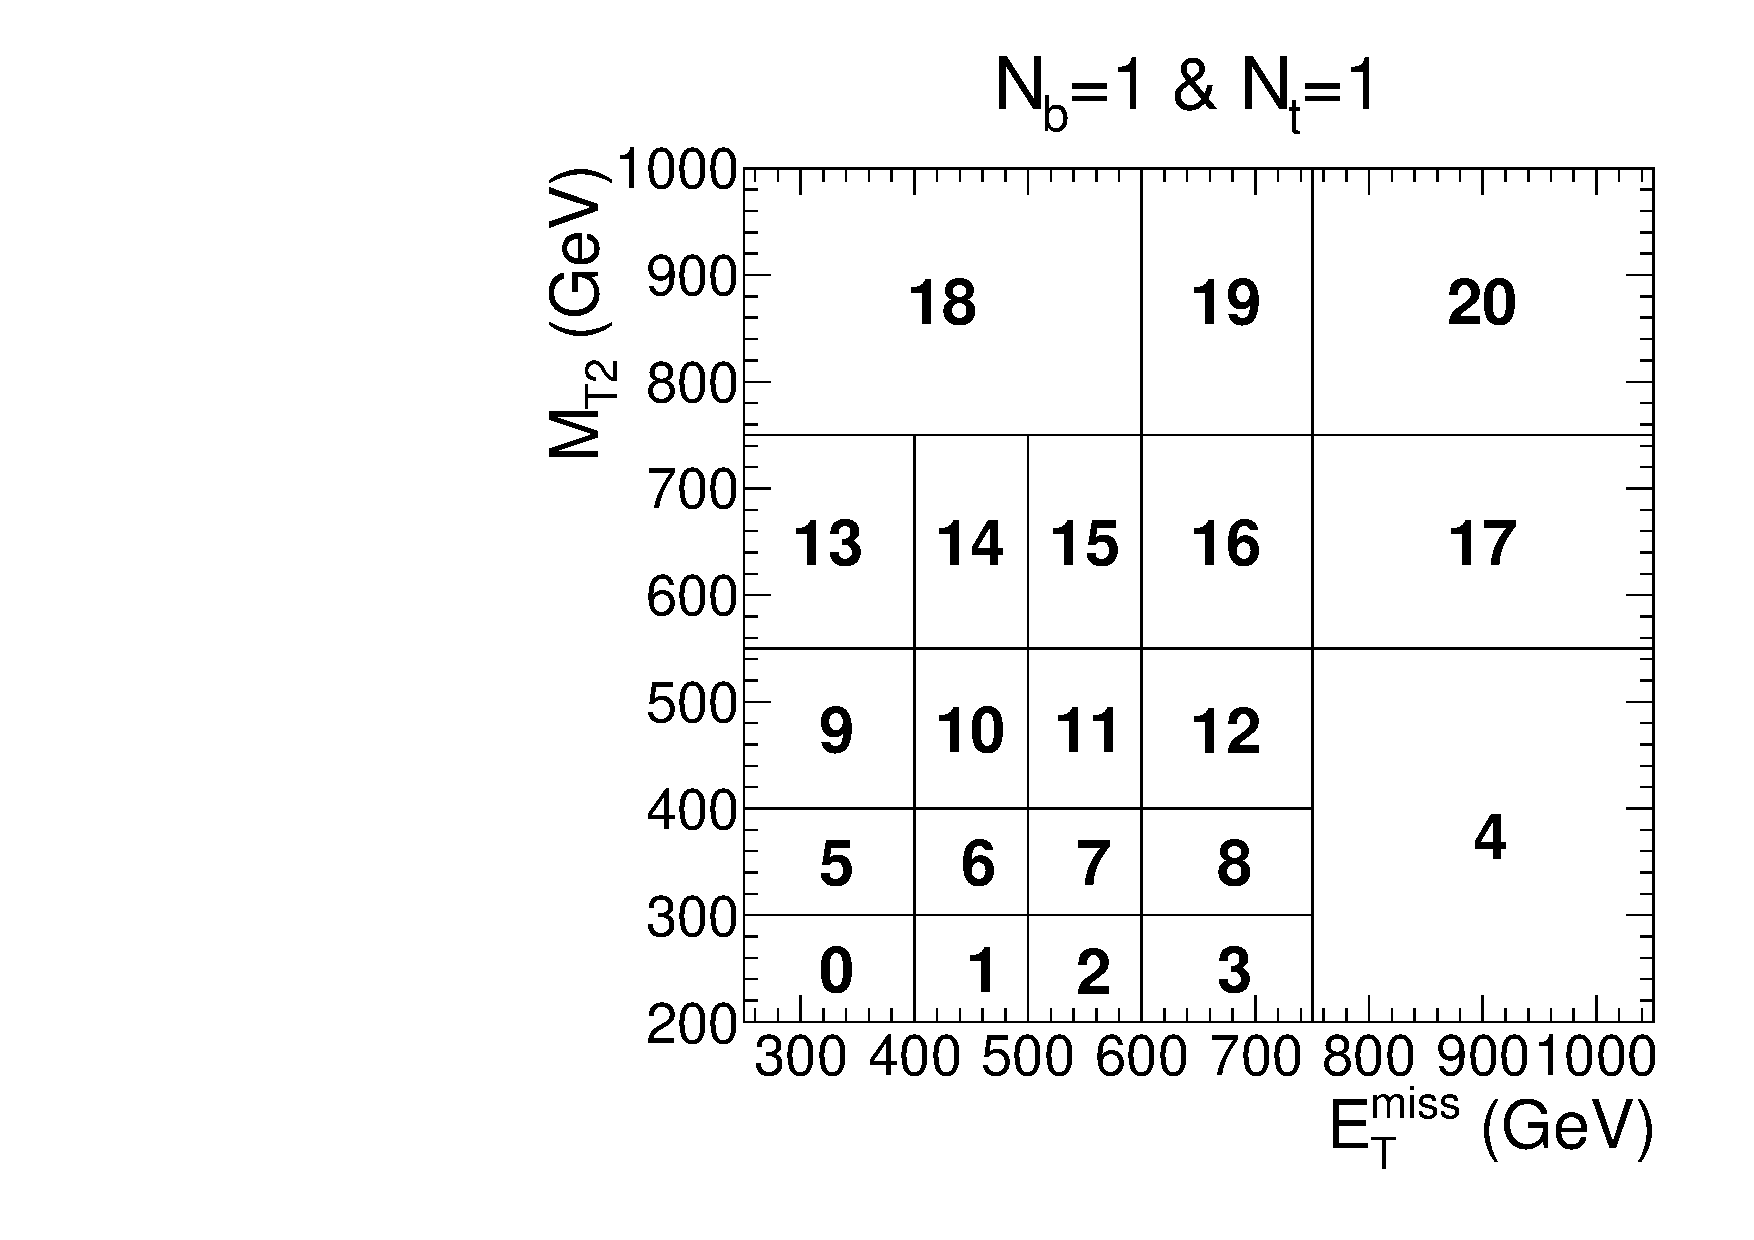
\includegraphics[width=0.30\linewidth]{sections/mc4/EvtSelSBOpt/figures/poly_MT2_vs_met_0.pdf}
    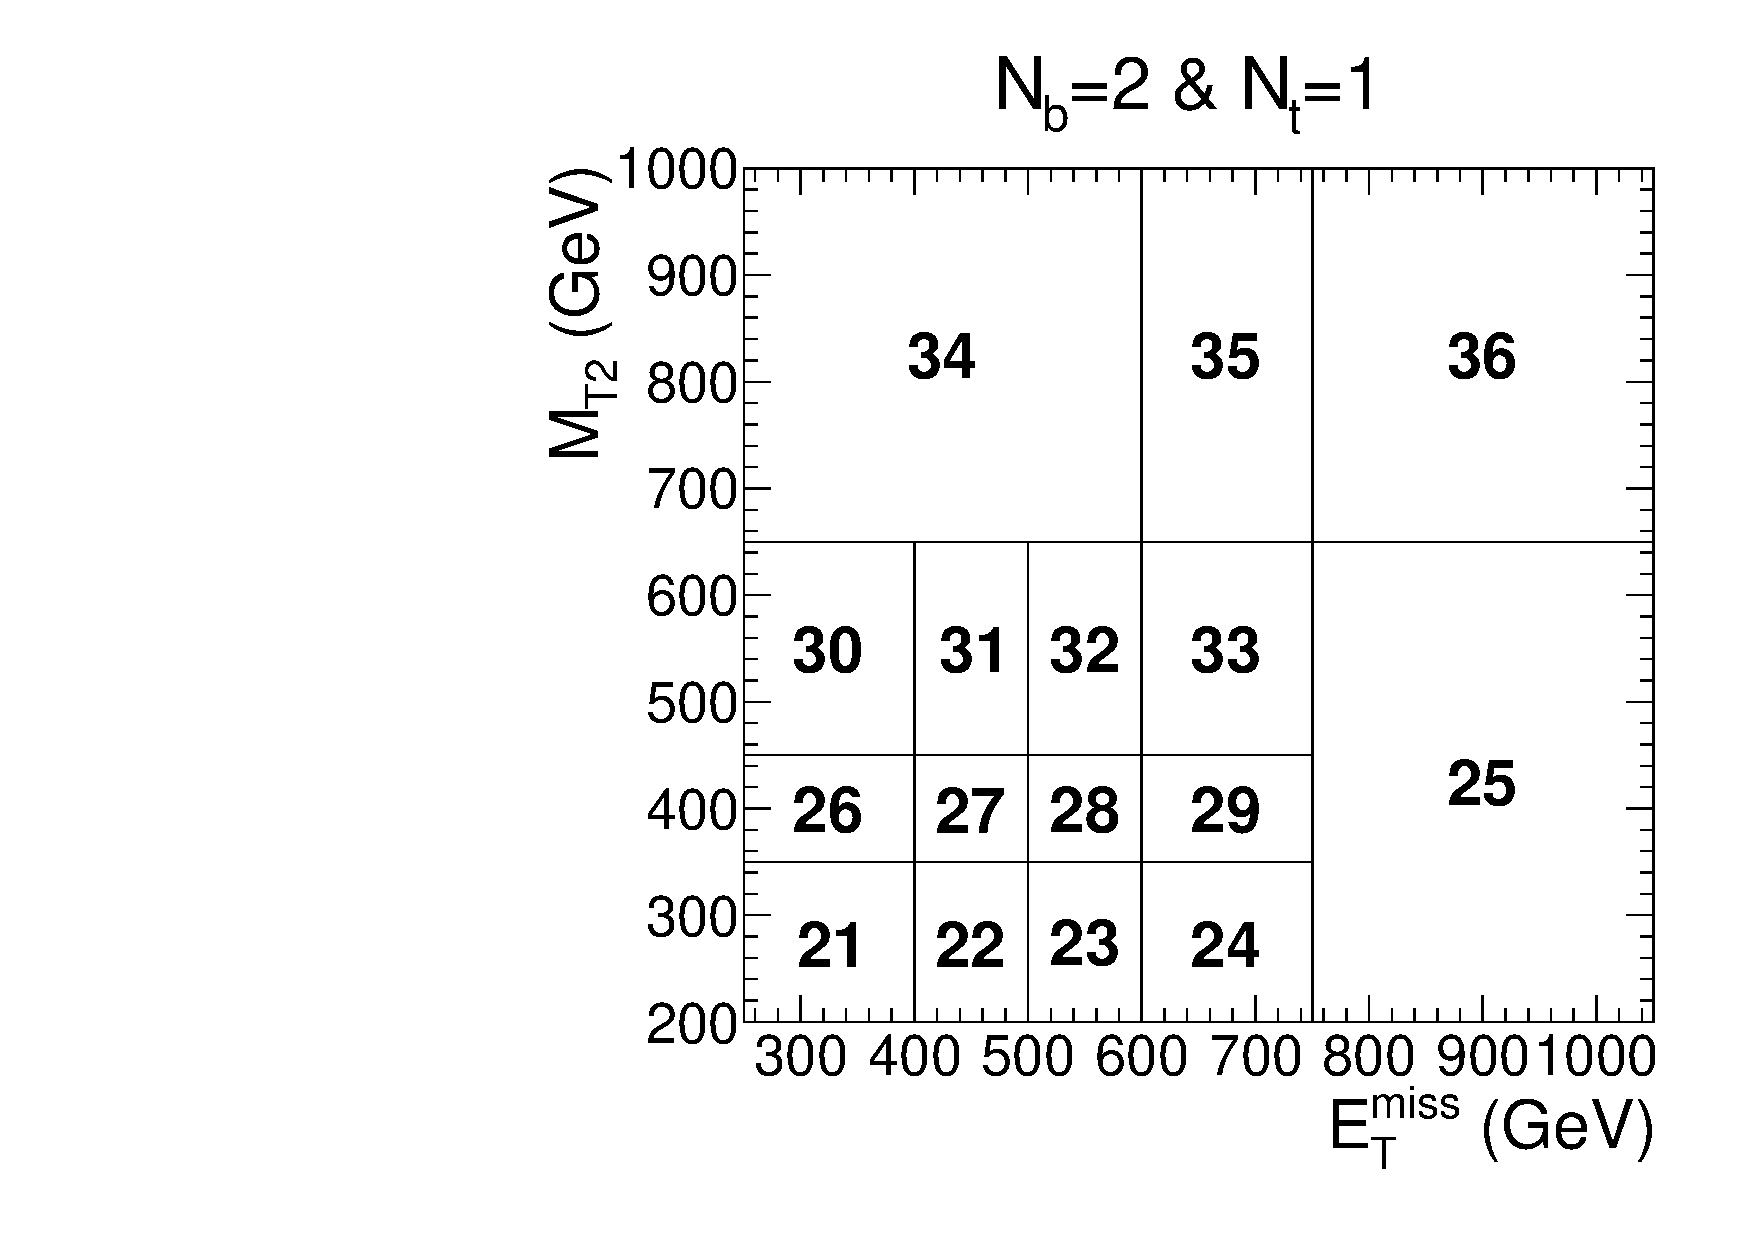
\includegraphics[width=0.30\linewidth]{sections/mc4/EvtSelSBOpt/figures/poly_MT2_vs_met_1.pdf}
    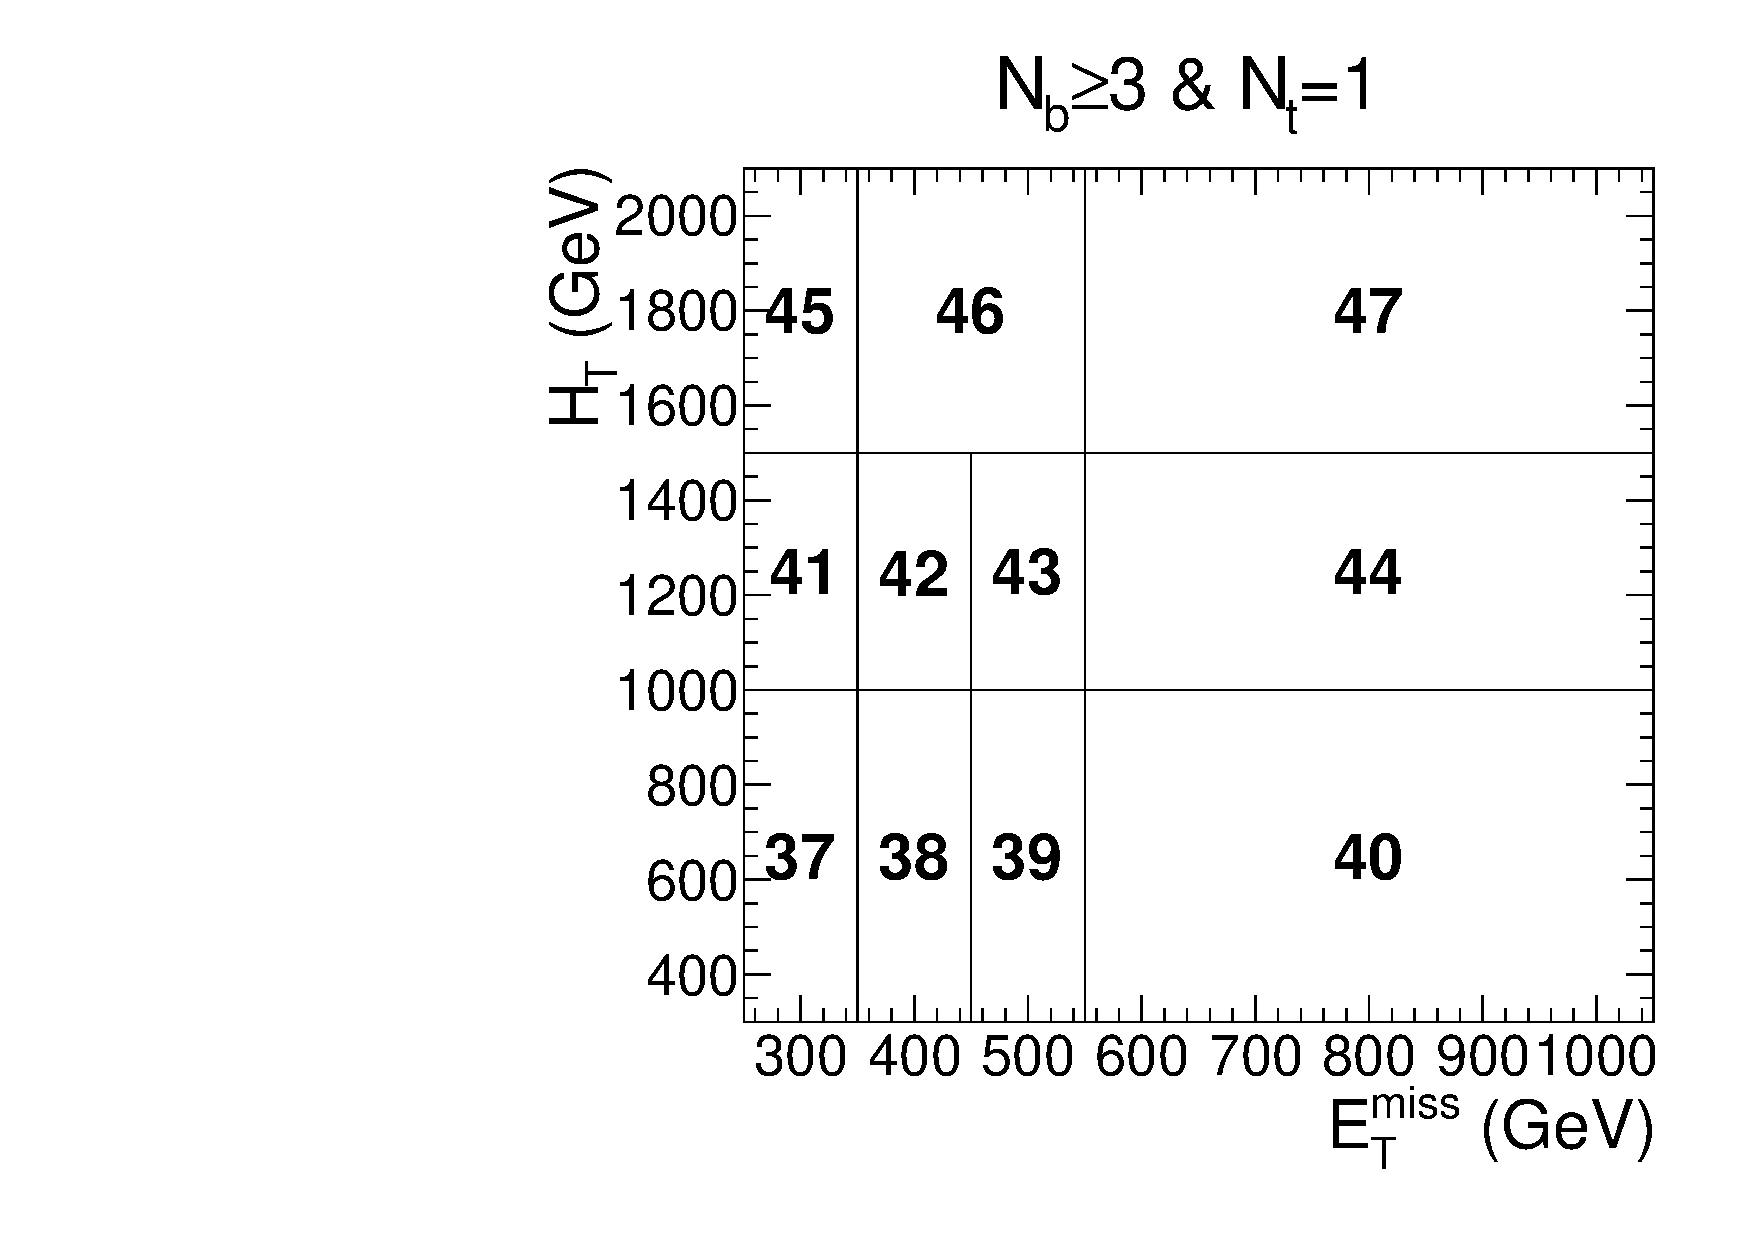
\includegraphics[width=0.30\linewidth]{sections/mc4/EvtSelSBOpt/figures/poly_MT2_vs_met_2.pdf} \\
    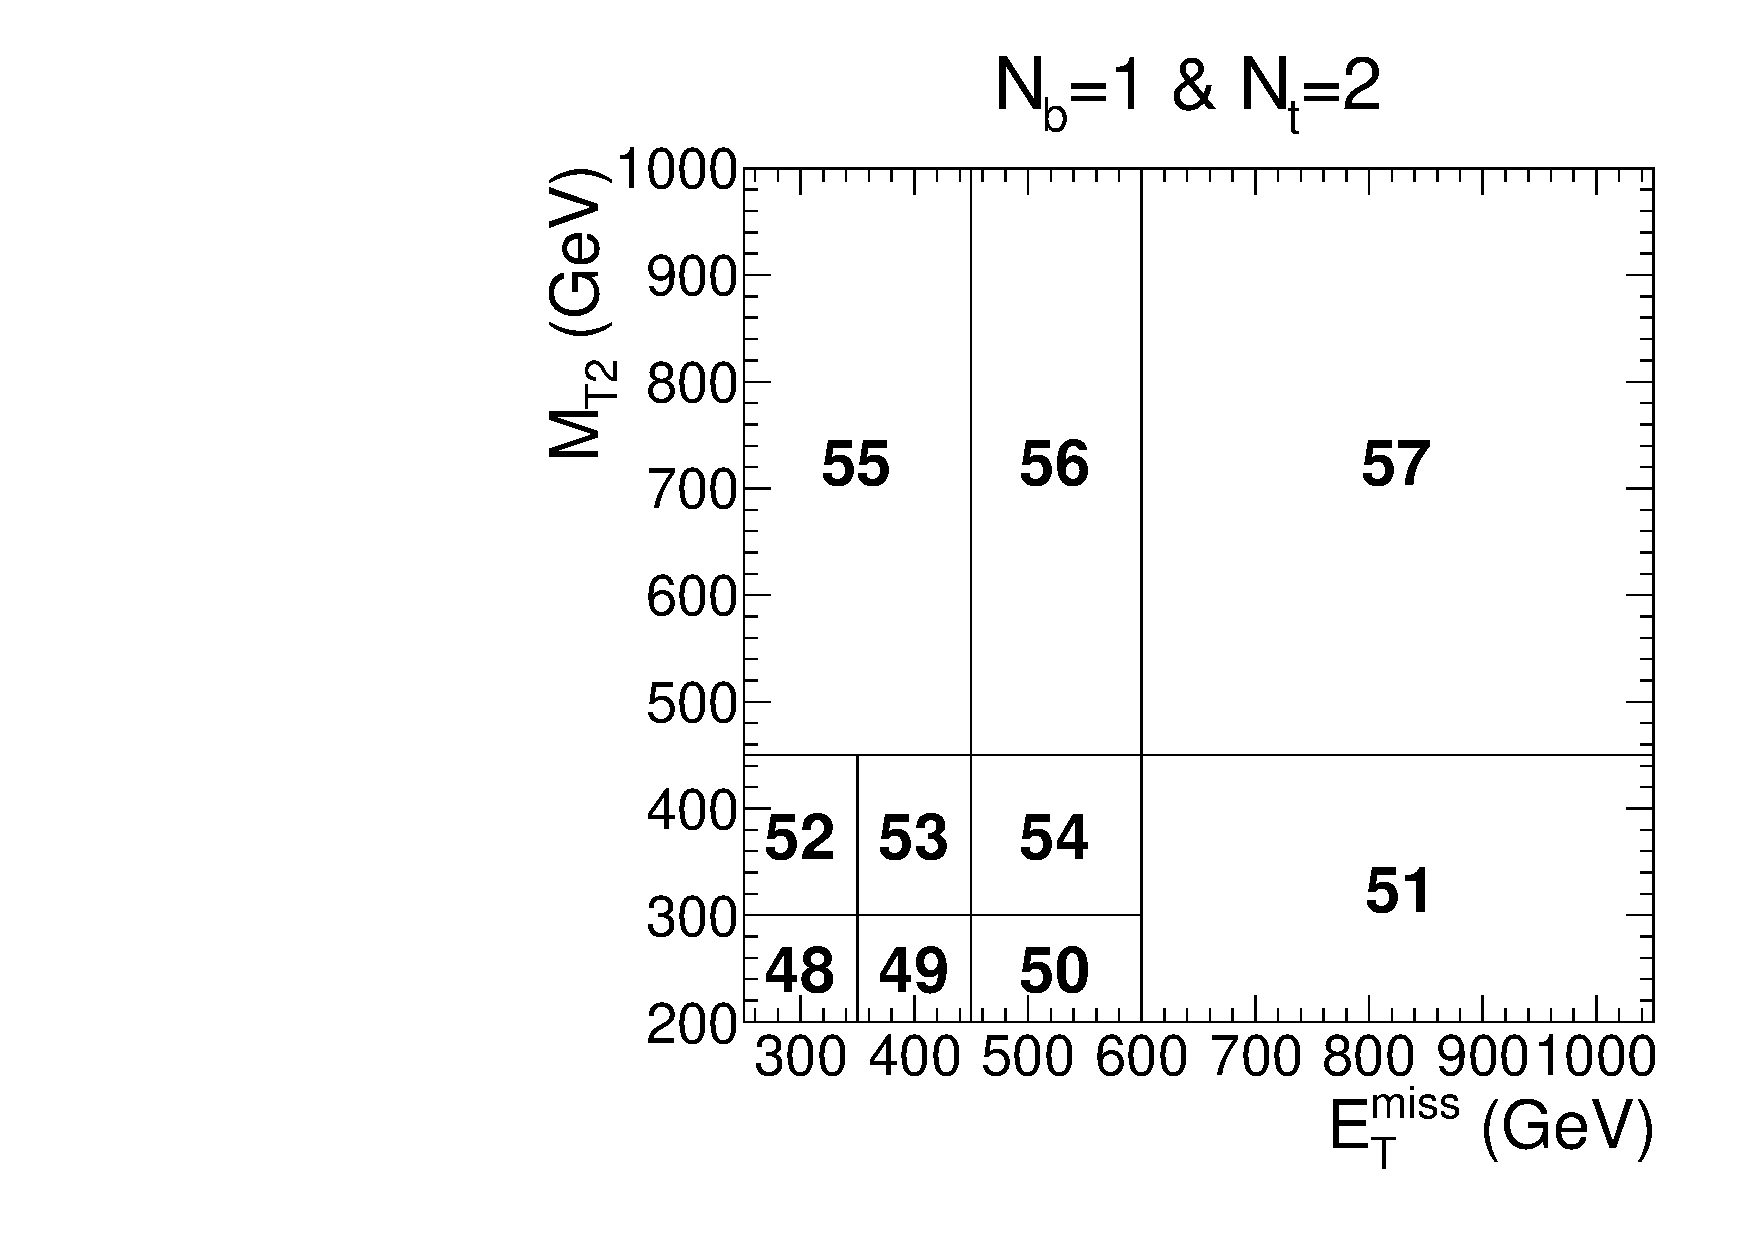
\includegraphics[width=0.30\linewidth]{sections/mc4/EvtSelSBOpt/figures/poly_MT2_vs_met_3.pdf} 
    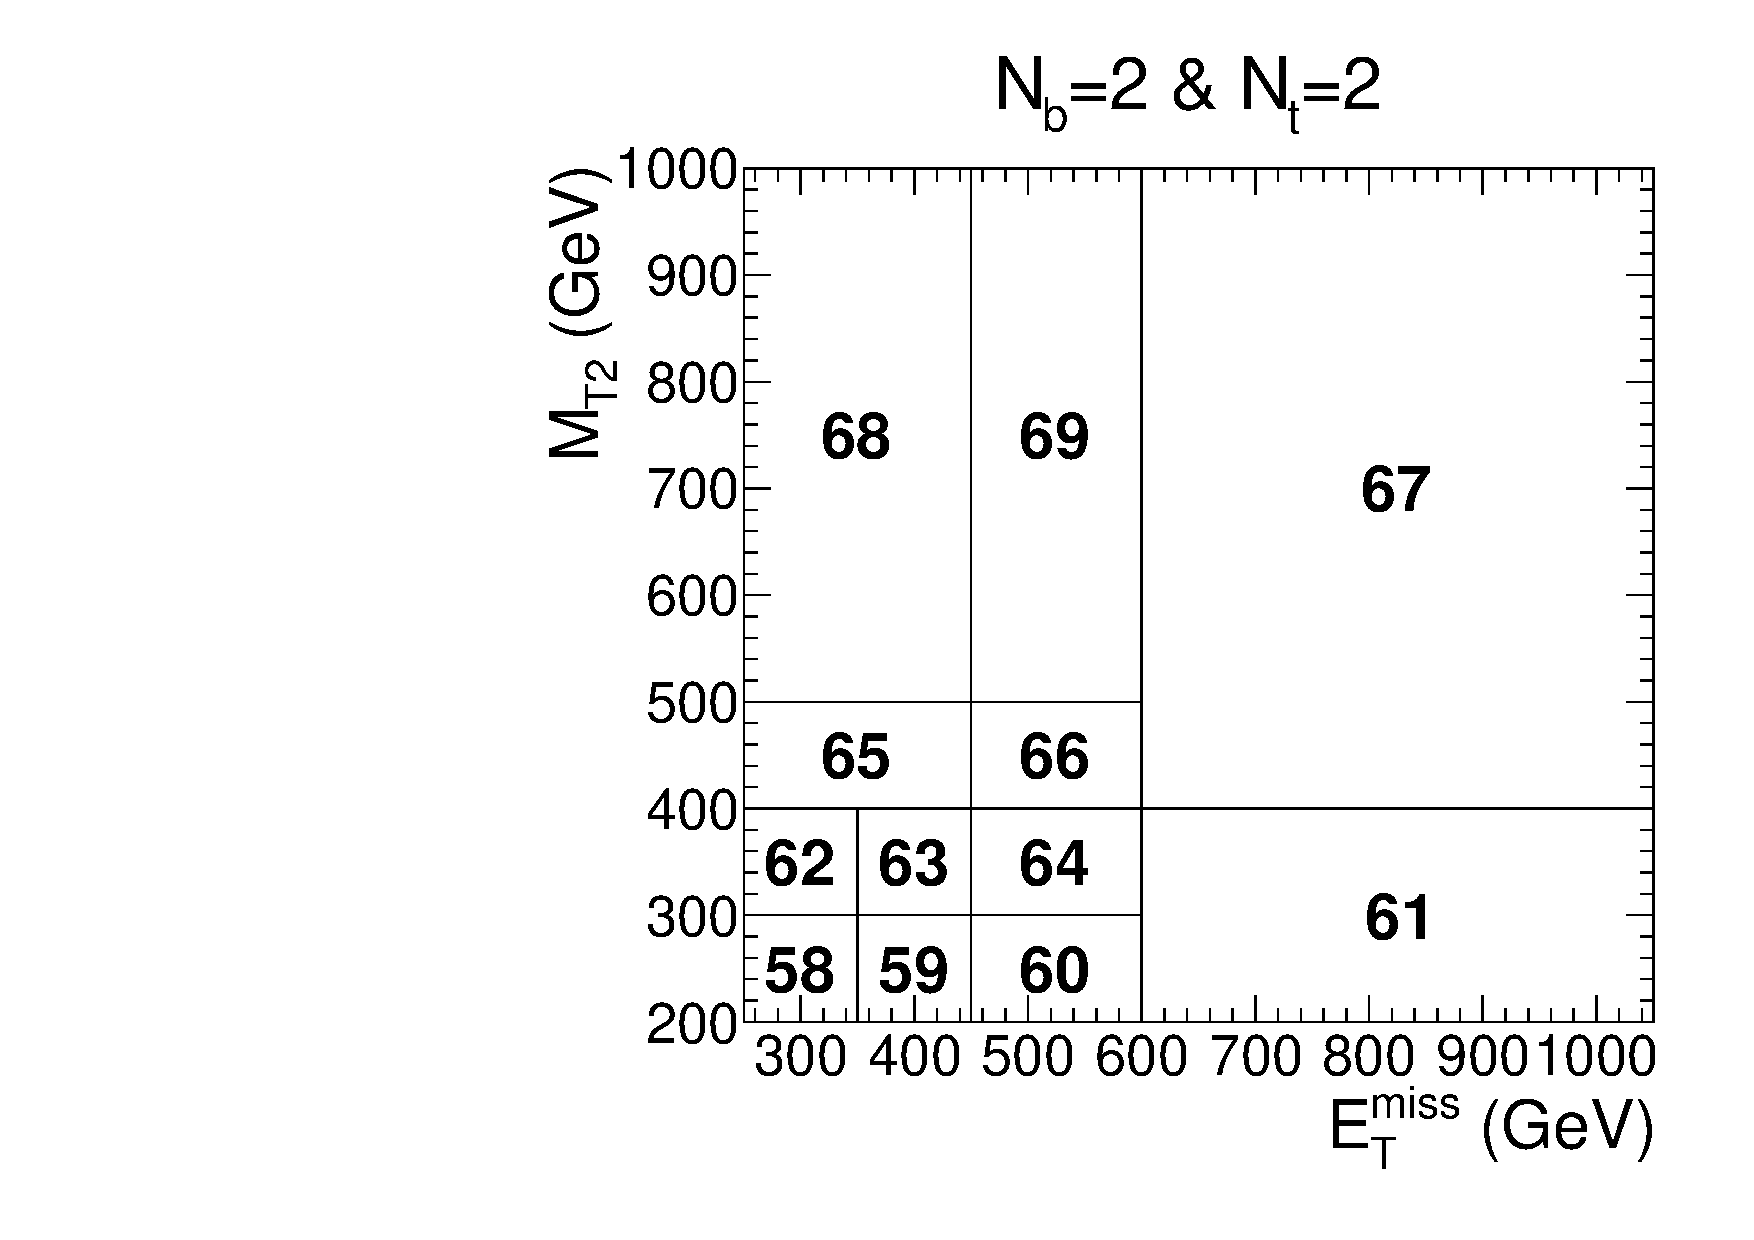
\includegraphics[width=0.30\linewidth]{sections/mc4/EvtSelSBOpt/figures/poly_MT2_vs_met_4.pdf} 
    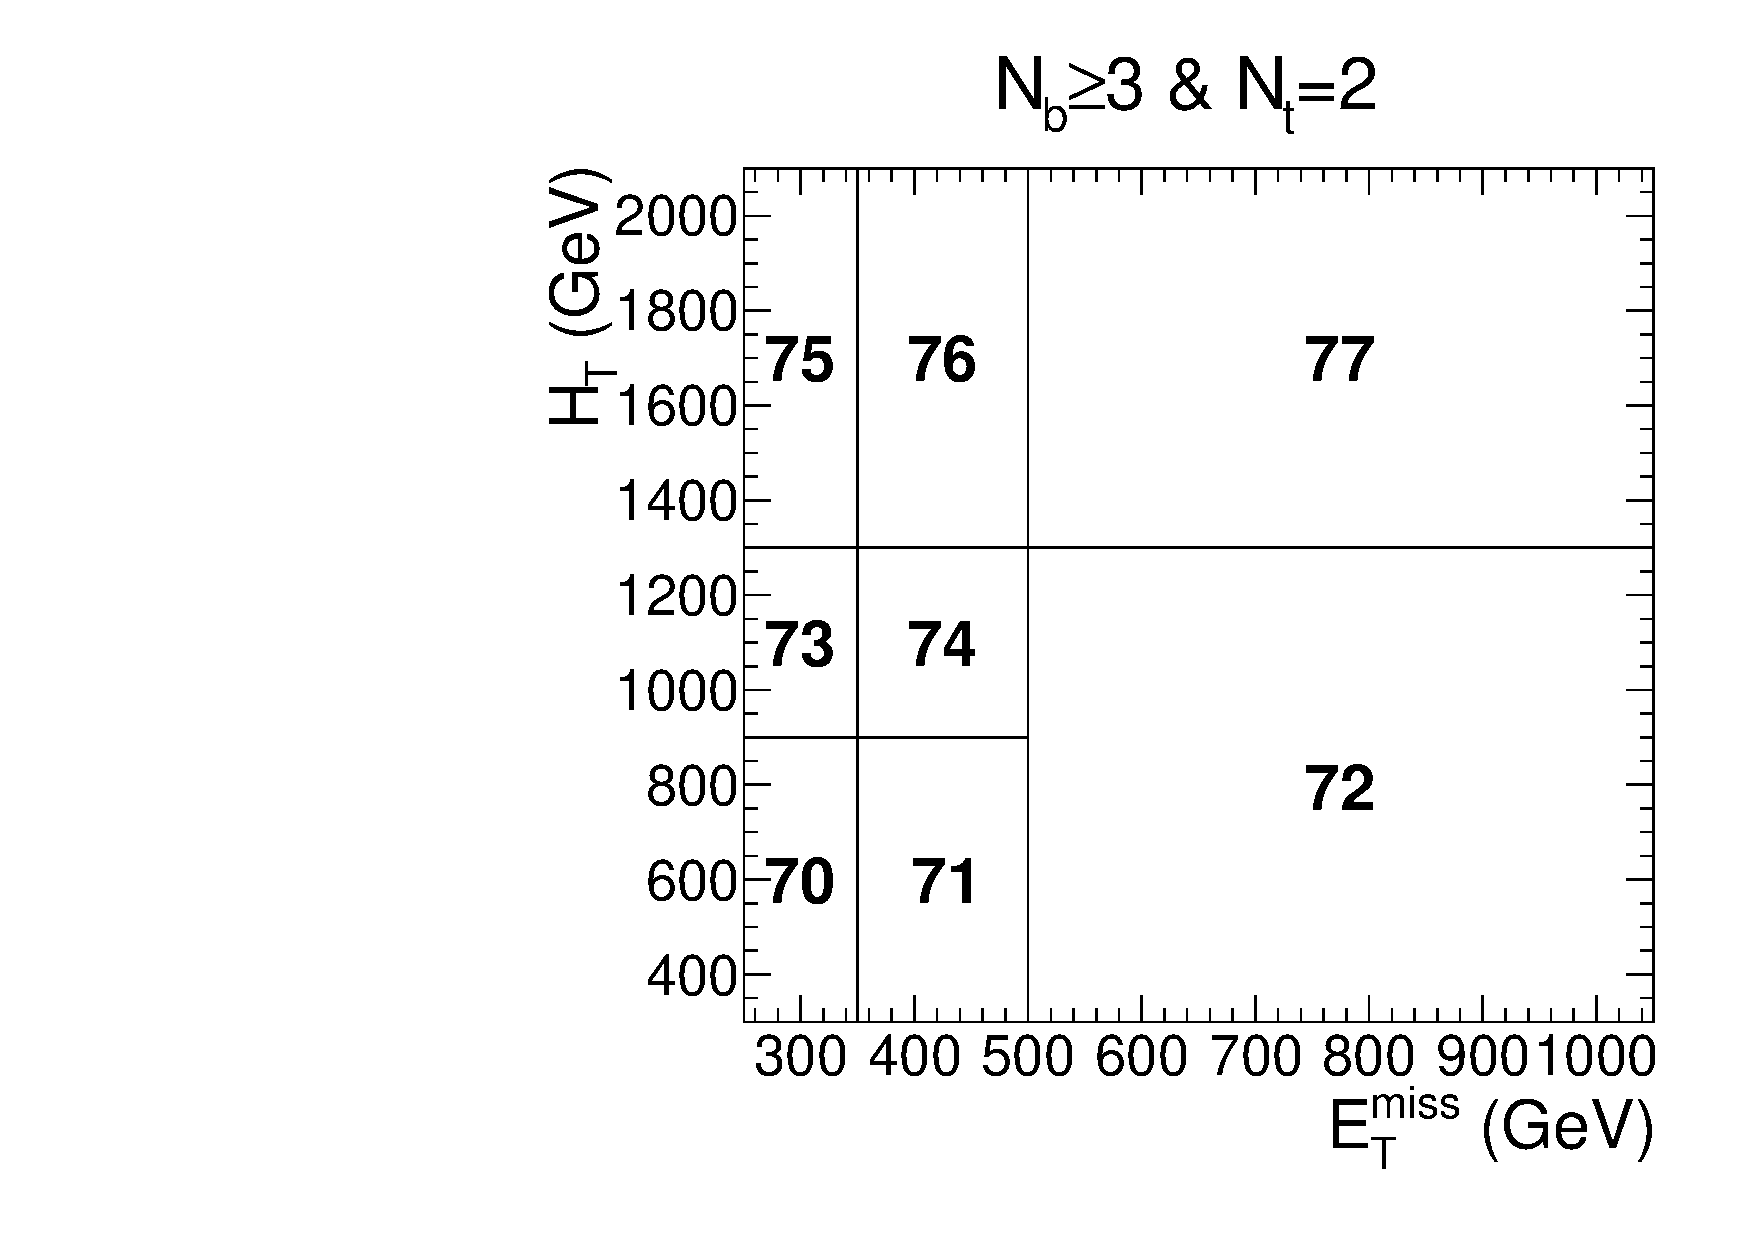
\includegraphics[width=0.30\linewidth]{sections/mc4/EvtSelSBOpt/figures/poly_MT2_vs_met_5.pdf} \\
    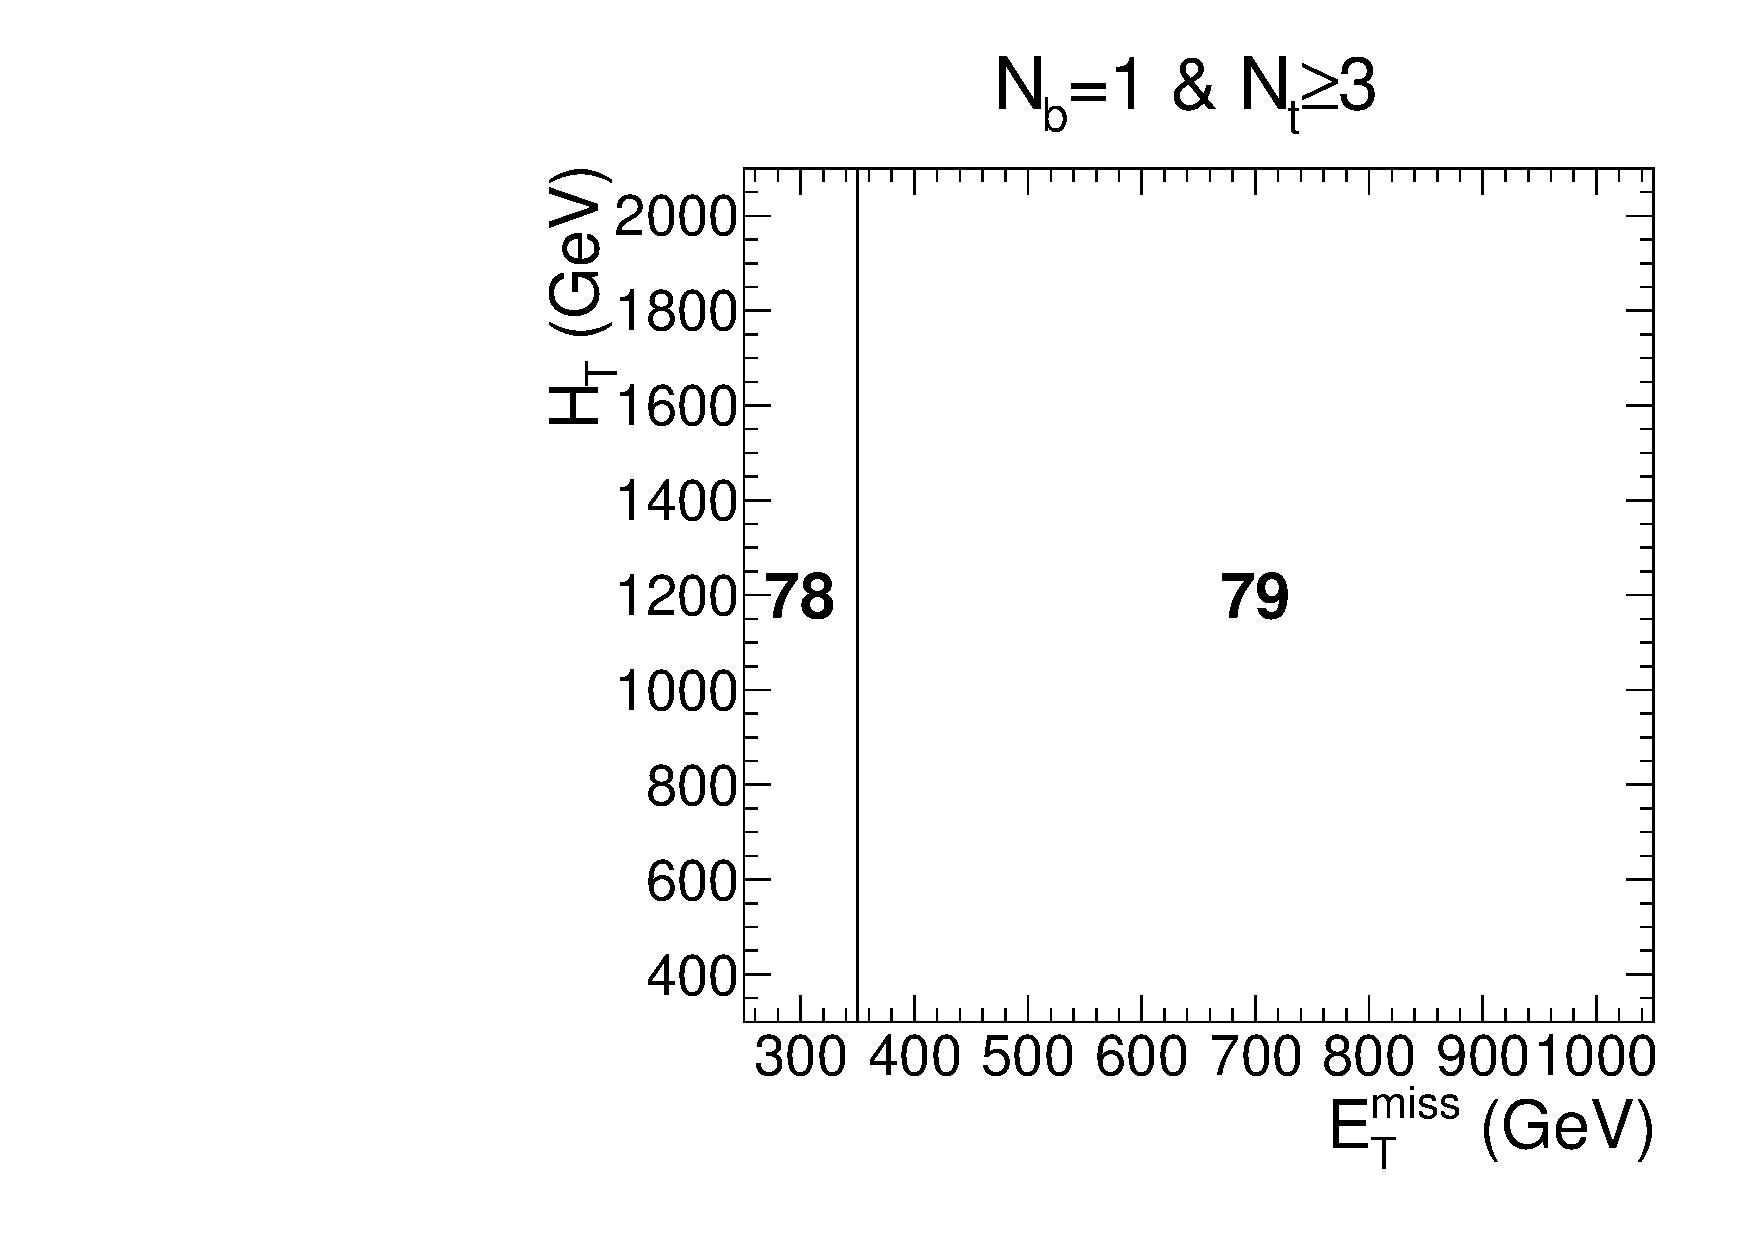
\includegraphics[width=0.30\linewidth]{sections/mc4/EvtSelSBOpt/figures/poly_MT2_vs_met_6.pdf} 
    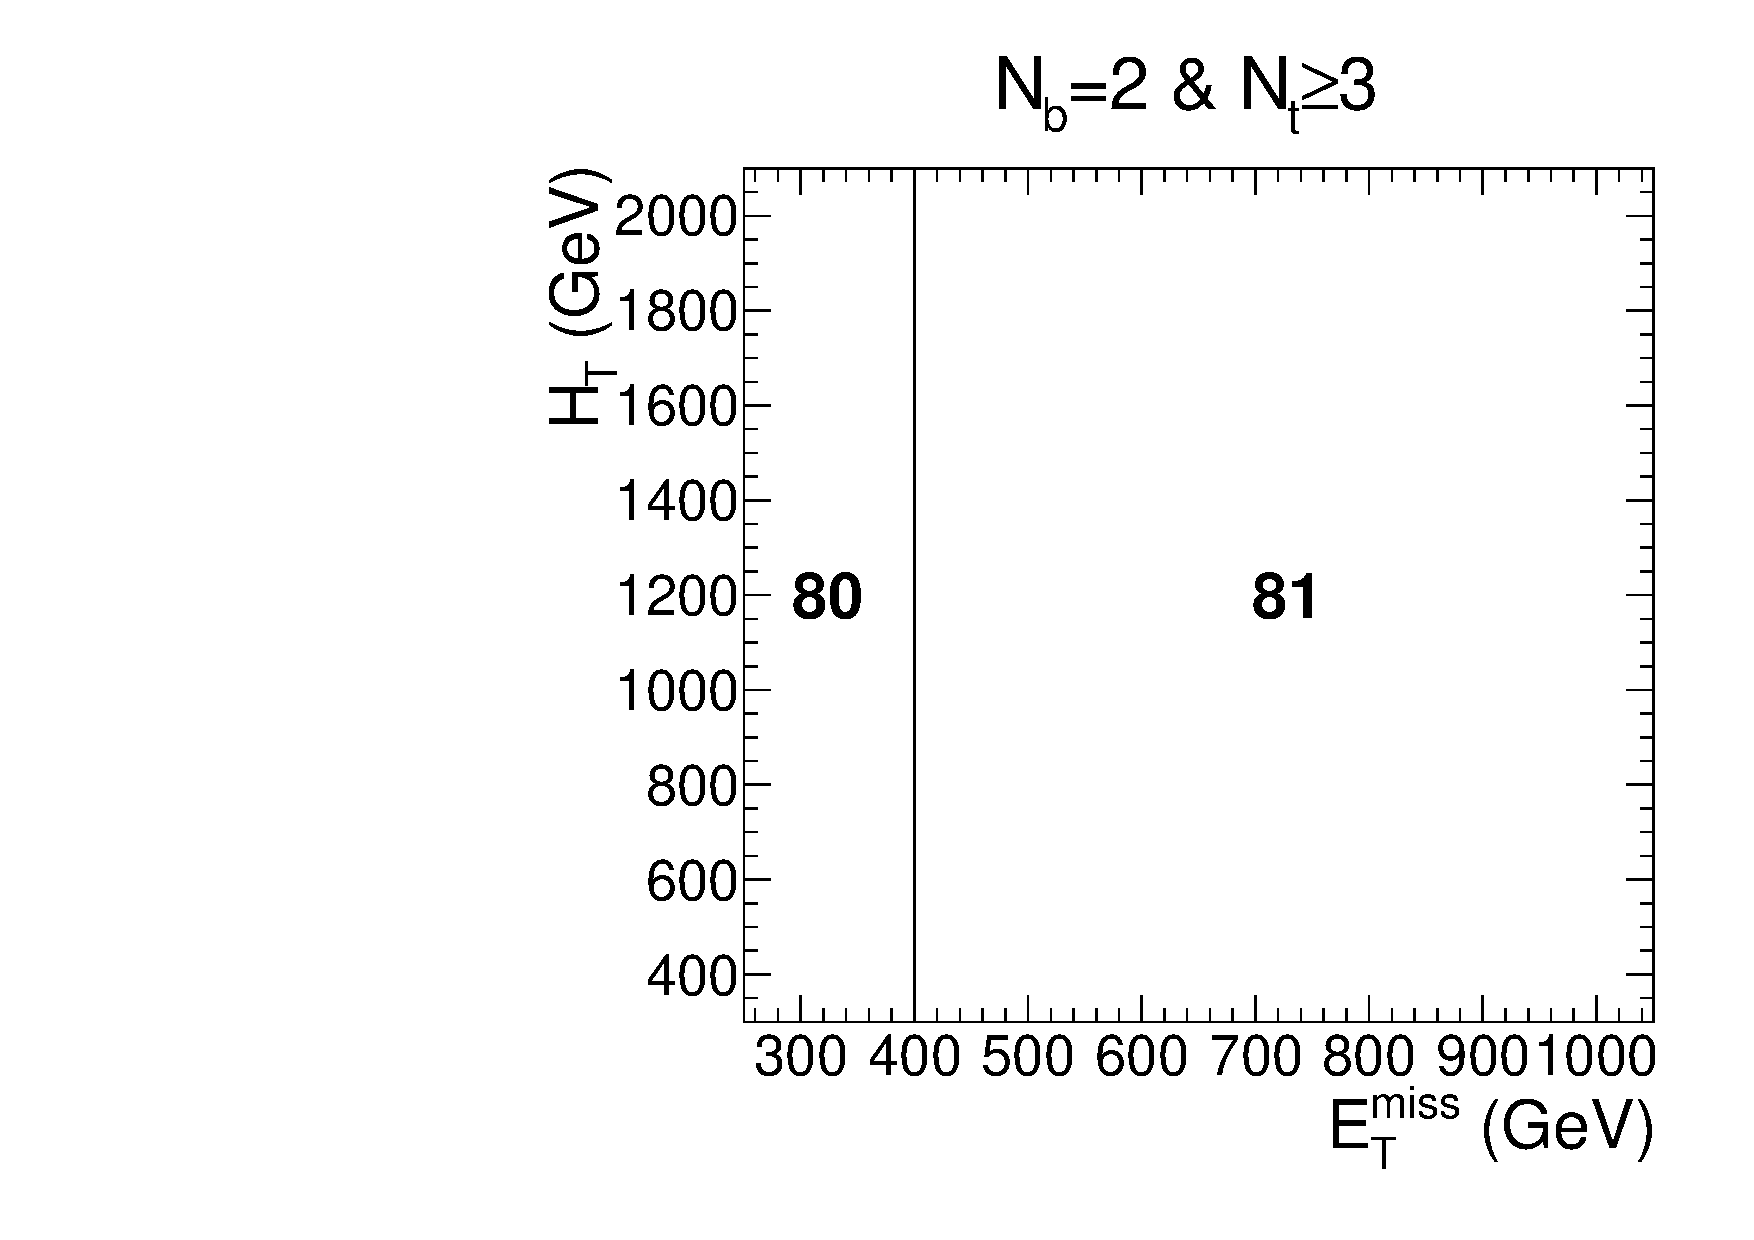
\includegraphics[width=0.30\linewidth]{sections/mc4/EvtSelSBOpt/figures/poly_MT2_vs_met_7.pdf} 
    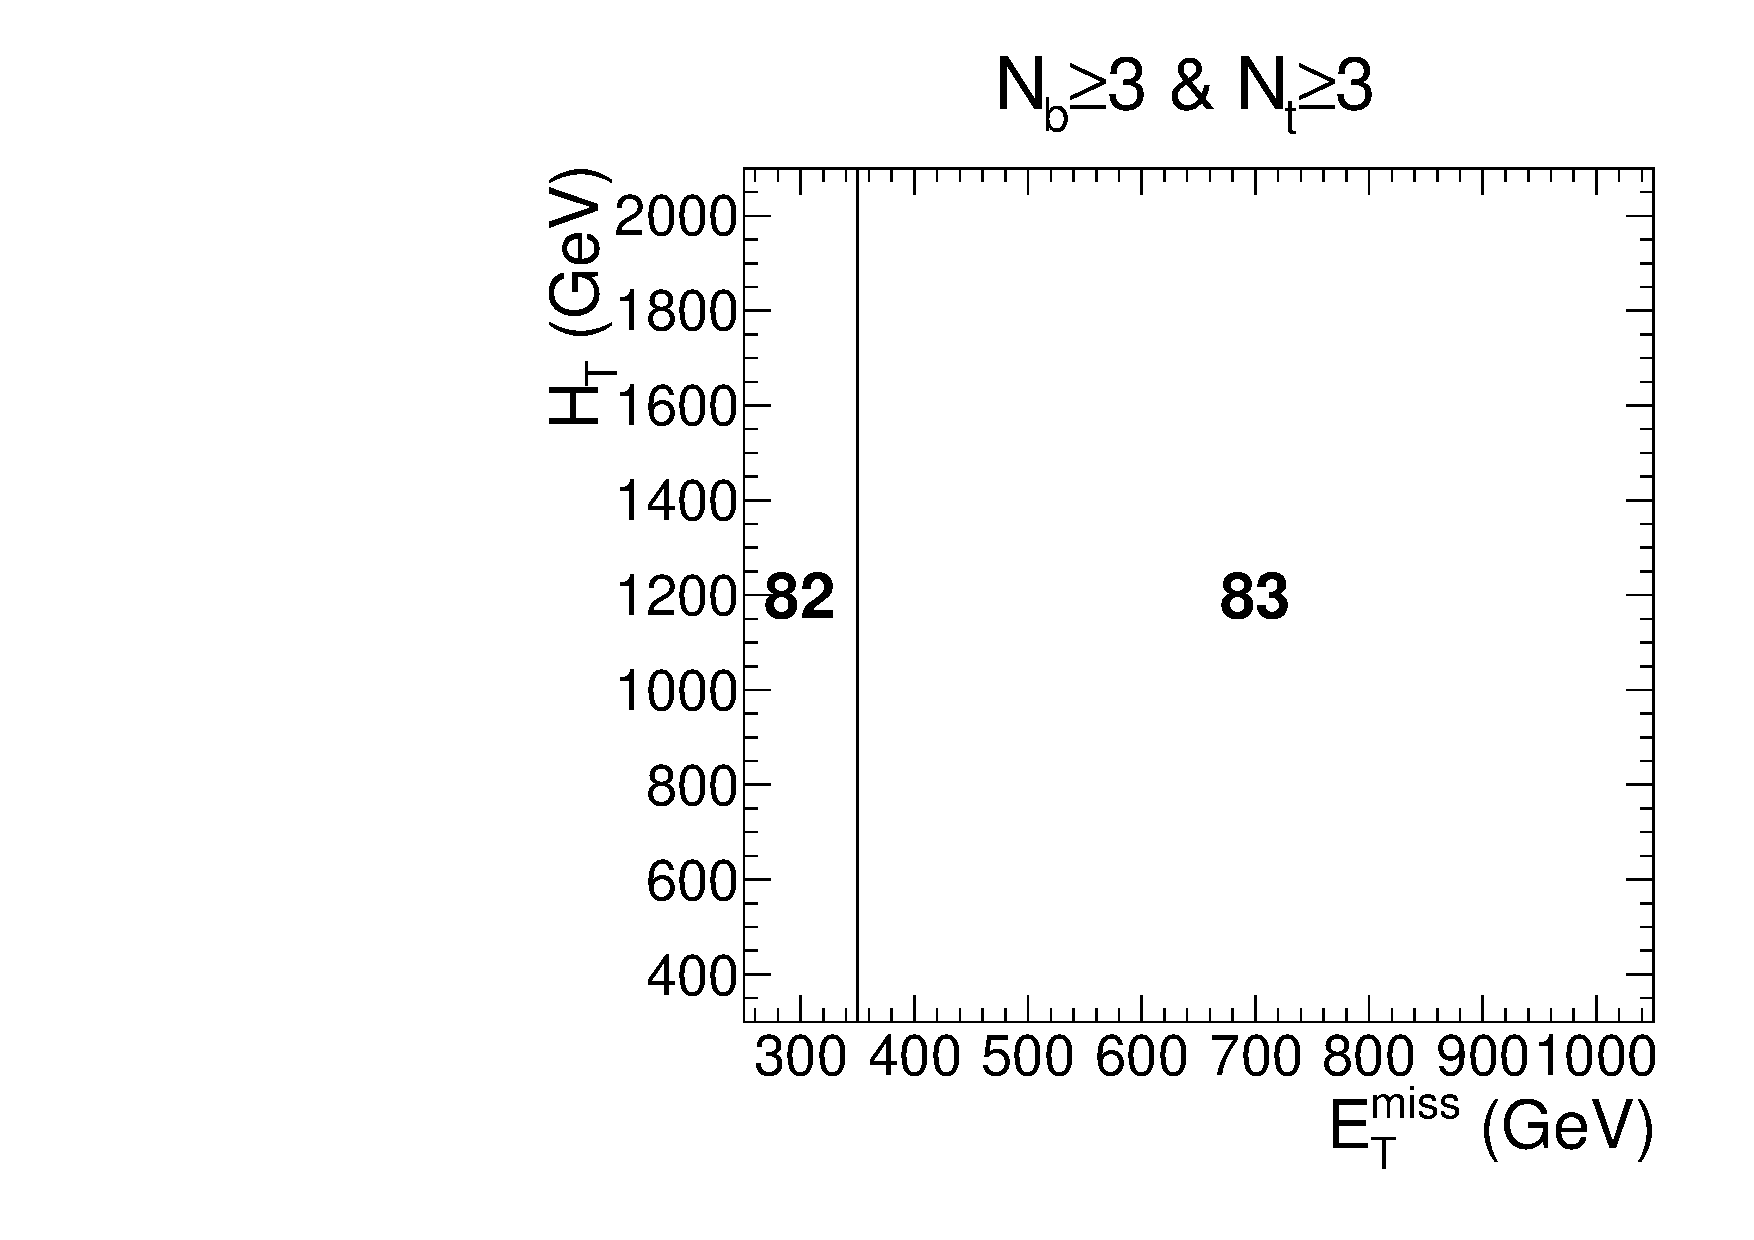
\includegraphics[width=0.30\linewidth]{sections/mc4/EvtSelSBOpt/figures/poly_MT2_vs_met_8.pdf} \\
    \caption{Original search bin definitions after baseline cuts (in total 84 search bins). }
    \label{fig:SBXX}
  \end{center}
\end{figure}

\subsection{MC samples for background and signal Studies}
\label{sec:sm-mc}

The analysis uses a set of Monte Carlo samples for background estimation method
development and predictions as well as SUSY signal samples for the interpretation
of the results. All the
background samples are generated with the Geant4-based CMS simulation 
application while all the signal samples for limit setting are generated
using the Fast Simulation application.

\paragraph{Standard Model Samples}

Monte Carlo samples of SM processes reconstructed with CMSSW release 8.0 (Summer16) are used in this thesis. A complete list of these samples is given in Table~\ref{tab:MCsamples1} and Table~\ref{tab:MCsamples2}. The cross sections listed come from calculations performed at the next-to-next-to-leading-order (NNLO) unless otherwise noted. All samples use the ``Moriond17" pileup scenario, which simulates a pileup distribution with an average of 25 interactions per bunch crossing and a 25~ns interval between bunches.

\begin{table}[hp]
\centering
\caption{Standard model Monte Carlo samples used in the analysis.}
\label{tab:MCsamples1}
{
%\scriptsize
\footnotesize
\begin{tabular}{lcc}
\hline \hline
Dataset & $\sigma$ (pb) \\
\hline
\multicolumn{2}{c}{QCD MC samples (LO)} \\ \hline
QCD\_HT100to200\_TuneCUETP8M1\_13TeV-madgraphMLM-pythia8 & 27540000 \\
QCD\_HT200to300\_TuneCUETP8M1\_13TeV-madgraphMLM-pythia8 & 1735000 \\
QCD\_HT300to500\_TuneCUETP8M1\_13TeV-madgraphMLM-pythia8 & 366800 \\
QCD\_HT500to700\_TuneCUETP8M1\_13TeV-madgraphMLM-pythia8 & 29370 \\
QCD\_HT700to1000\_TuneCUETP8M1\_13TeV-madgraphMLM-pythia8 & 6524 \\
QCD\_HT1000to1500\_TuneCUETP8M1\_13TeV-madgraphMLM-pythia8 & 1064 \\
QCD\_HT1500to2000\_TuneCUETP8M1\_13TeV-madgraphMLM-pythia8 & 121.5 \\
QCD\_HT2000toInf\_TuneCUETP8M1\_13TeV-madgraphMLM-pythia8 & 25.42 \\
\hline
\multicolumn{2}{c}{SM \ttbar MC samples} \\ \hline
TTJets\_TuneCUETP8M1\_13TeV-madgraphMLM-pythia8 & 816.0 \\
TTJets\_SingleLeptFromT\_TuneCUETP8M1\_13TeV-madgraphMLM-pythia8 & 179.3 \\
TTJets\_SingleLeptFromTbar\_TuneCUETP8M1\_13TeV-madgraphMLM-pythia8 & 179.3 \\
TTJets\_DiLept\_TuneCUETP8M1\_13TeV-madgraphMLM-pythia8 & 86.66 \\
TTJets\_HT-600to800\_TuneCUETP8M1\_13TeV-madgraphMLM-pythia8 & 2.615 \\
TTJets\_HT-800to1200\_TuneCUETP8M1\_13TeV-madgraphMLM-pythia8 & 1.077 \\
TTJets\_HT-1200to2500\_TuneCUETP8M1\_13TeV-madgraphMLM-pythia8 & 0.195 \\
TTJets\_HT-2500toInf\_TuneCUETP8M1\_13TeV-madgraphMLM-pythia8 & 0.002 \\
\hline
\multicolumn{2}{c}{SM \wlnu MC samples} \\ \hline
WJetsToLNu\_HT-100To200\_TuneCUETP8M1\_13TeV-madgraphMLM-pythia8 & 1635 \\
WJetsToLNu\_HT-200To400\_TuneCUETP8M1\_13TeV-madgraphMLM-pythia8 & 437.0 \\
WJetsToLNu\_HT-400To600\_TuneCUETP8M1\_13TeV-madgraphMLM-pythia8 & 59.50 \\
WJetsToLNu\_HT-600ToInf\_TuneCUETP8M1\_13TeV-madgraphMLM-pythia8 & 22.80 \\
WJetsToLNu\_HT-600To800\_TuneCUETP8M1\_13TeV-madgraphMLM-pythia8 & 15.50 \\
WJetsToLNu\_HT-800To1200\_TuneCUETP8M1\_13TeV-madgraphMLM-pythia8 & 6.366 \\
WJetsToLNu\_HT-1200To2500\_TuneCUETP8M1\_13TeV-madgraphMLM-pythia8 & 1.614 \\
WJetsToLNu\_HT-2500ToInf\_TuneCUETP8M1\_13TeV-madgraphMLM-pythia8 & 0.037 \\
\hline \hline
\end{tabular}
}
\end{table}

\begin{table}[hp]
\centering
\caption{Standard model Monte Carlo samples used in the analysis.}
\label{tab:MCsamples2}
{
%\scriptsize
\footnotesize
\begin{tabular}{lcc}
\hline \hline
Dataset & $\sigma$ (pb) \\
\hline
\multicolumn{2}{c}{SM \znunu MC samples} \\ \hline
ZJetsToNuNu\_HT-100To200\_13TeV-madgraph & 345.0 \\
ZJetsToNuNu\_HT-200To400\_13TeV-madgraph & 96.38 \\
ZJetsToNuNu\_HT-400To600\_13TeV-madgraph & 13.46 \\
ZJetsToNuNu\_HT-600ToInf\_13TeV-madgraph & 5.170 \\
ZJetsToNuNu\_HT-600To800\_13TeV-madgraph & 3.146 \\
ZJetsToNuNu\_HT-800To1200\_13TeV-madgraph & 1.453 \\
ZJetsToNuNu\_HT-1200To2500\_13TeV-madgraph & 0.359 \\
ZJetsToNuNu\_HT-2500ToInf\_13TeV-madgraph & 0.0085 \\
\hline
\multicolumn{2}{c}{SM \zll MC samples} \\ \hline
DYJetsToLL\_M-50\_TuneCUETP8M1\_13TeV-madgraphMLM-pythia8 & 6025 \\
DYJetsToLL\_M-50\_HT-100to200\_TuneCUETP8M1\_13TeV-madgraphMLM-pythia8 & 171.5 \\
DYJetsToLL\_M-50\_HT-200to400\_TuneCUETP8M1\_13TeV-madgraphMLM-pythia8 & 52.58 \\
DYJetsToLL\_M-50\_HT-400to600\_TuneCUETP8M1\_13TeV-madgraphMLM-pythia8 & 6.984 \\
DYJetsToLL\_M-50\_HT-600to800\_TuneCUETP8M1\_13TeV-madgraphMLM-pythia8 & 1.676 \\
DYJetsToLL\_M-50\_HT-800to1200\_TuneCUETP8M1\_13TeV-madgraphMLM-pythia8 & 0.831 \\
DYJetsToLL\_M-50\_HT-1200to2500\_TuneCUETP8M1\_13TeV-madgraphMLM-pythia8 & 0.143 \\
DYJetsToLL\_M-50\_HT-2500toInf\_TuneCUETP8M1\_13TeV-madgraphMLM-pythia8 & 0.0032 \\
\hline
\multicolumn{2}{c}{SM single-top MC samples} \\ \hline
ST\_tW\_antitop\_5f\_inclusiveDecays\_13TeV-powheg-pythia8\_TuneCUETP8M1 & 35.80\\
ST\_tW\_top\_5f\_inclusiveDecays\_13TeV-powheg-pythia8\_TuneCUETP8M1 & 35.80\\
\hline
\multicolumn{2}{c}{SM di-boson and other rare process MC samples} \\ \hline
ttHJetTobb\_M125\_13TeV\_amcatnloFXFX\_madspin\_pythia8 & 0.293 \\
TTZToLLNuNu\_M-10\_TuneCUETP8M1\_13TeV-amcatnlo-pythia8 & 0.228 \\
TTZToQQ\_TuneCUETP8M1\_13TeV-amcatnlo-pythia8 & 0.530 \\
TTWJetsToLNu\_TuneCUETP8M1\_13TeV-amcatnloFXFX-madspin-pythia8 & 0.204 \\
TTWJetsToQQ\_TuneCUETP8M1\_13TeV-amcatnloFXFX-madspin-pythia8 & 0.423 \\
WW\_TuneCUETP8M1\_13TeV\_pythia8 & 115.0 \\
WZ\_TuneCUETP8M1\_13TeV\_pythia8 & 47.13 \\
ZZ\_TuneCUETP8M1\_13TeV\_pythia8 & 16.523 \\
WWZ\_TuneCUETP8M1\_13TeV-amcatnlo-pythia8 & 0.165 \\
WZZ\_TuneCUETP8M1\_13TeV-amcatnlo-pythia8 & 0.056 \\
ZZZ\_TuneCUETP8M1\_13TeV-amcatnlo-pythia8 & 0.014 \\
\hline \hline
\end{tabular}
}
\end{table}

\paragraph{Signal samples}

Diagrams associated with the signal simplified models (SMS) used in this search for interpretation of the results are shown in Fig~\ref{fig:signal_diagrams}. The top diagram is often referred to as T2tt($x,y$) and represents direct squark-antisquark pair production with $x$ and $y$ the top squark and \chiOneZero masses, respectively~\cite{CMS-SMS-paper}. Under the assumption that the SUSY particles that could decay to top squarks are too heavy and beyond the reach of LHC Run 2, this diagram would represent the dominant process for top squark pair production and the target signal process for this analysis.

If the gluino is within the LHC reach in Run 2, gluino-induced processes such as those in the middle and bottom row of Fig~\ref{fig:signal_diagrams} would become relevant to the analysis. The middle left diagram is called T1tttt($x,y$) with $x$ and $y$ the gluino and \chiOneZero masses.
In this model, the gluino undergoes a three-body decay into \ensuremath{\rm t}, \ensuremath{\rm \bar{t}} and 
\chiOneZero. The event kinematics are similar to the case
where
$\gluino\to\mathrm{t}\sTop, \sTop\to\mathrm{t}\chiOneZero$~\cite{CMS-SMS-paper}
as in another model shown on the bottom right, denoted as T5ttcc($x,y,z$). The numbers in parentheses refer to the gluino, top squark, and 
\chiOneZero masses. 

Cross sections for a couple of mass points are shown in Table~\ref{tab:signalMC} for the T2tt and T1tttt SMS. These selected points were generated with full simulation and were used for cut flow studies and search region optimization. Limit setting was performed using fast simulation signal samples.

\begin{table}[hp]
\centering
\caption{Cross sections for a couple of mass points for the T2tt and T1tttt Simplified Models. The selected points were generated with full simulation.} %Note that all samples are generated with FullSim.}
\label{tab:signalMC}
{\footnotesize
\begin{tabular}{lcc}
\hline \hline
Dataset & $\sigma$ (pb) \\
\hline
SMS-T2tt\_mStop-500\_mLSP-325\_TuneCUETP8M1\_13TeV-madgraph-pythia8 & 0.51848 \\
SMS-T2tt\_mStop-850\_mLSP-100\_TuneCUETP8M1\_13TeV-madgraphMLM-pythia8 & 0.01896 \\
\hline
SMS-T1tttt\_mGluino-1500\_mLSP-100\_TuneCUETP8M1\_13TeV-madgraph-pythia8 & 0.014 \\
SMS-T1tttt\_mGluino-1200\_mLSP-800\_TuneCUETP8M1\_13TeV-madgraph-pythia8 & 0.086 \\
\hline \hline
\end{tabular}
\footnotesize}
\end{table}

